\documentclass{article}

% if you need to pass options to natbib, use, e.g.:
%     \PassOptionsToPackage{numbers, compress}{natbib}
% before loading neurips_2026

% 0. "default" for submission (Main Track, double-blind)
% \usepackage{neurips_2026}
% After being accepted:
% \usepackage[main, final]{neurips_2026}
% For preprint:
\usepackage[preprint]{neurips_2026}

\usepackage[utf8]{inputenc} % allow utf-8 input
\usepackage[T1]{fontenc}    % use 8-bit T1 fonts
\usepackage{hyperref}       % hyperlinks
\usepackage{url}            % simple URL typesetting
\usepackage{booktabs}       % professional-quality tables
\usepackage{amsfonts}       % blackboard math symbols
\usepackage{nicefrac}       % compact symbols for 1/2, etc.
\usepackage{microtype}      % microtypography
\usepackage{xcolor}         % colors

% Additional packages from the paper
\usepackage{graphicx}
\usepackage{subcaption}
\usepackage{xspace}
\usepackage{amsmath}
\usepackage{amssymb}
\usepackage{mathtools}
\usepackage{amsthm}
\usepackage{multirow}
\usepackage{float}
\usepackage{algorithm}
\usepackage{algpseudocode}

% if you use cleveref..
\usepackage[capitalize,noabbrev]{cleveref}

%%%%%%%%%%%%%%%%%%%%%%%%%%%%%%%%
% THEOREMS
%%%%%%%%%%%%%%%%%%%%%%%%%%%%%%%%
\theoremstyle{plain}
\newtheorem{theorem}{Theorem}[section]
\newtheorem{proposition}[theorem]{Proposition}
\newtheorem{lemma}[theorem]{Lemma}
\newtheorem{corollary}[theorem]{Corollary}
\theoremstyle{definition}
\newtheorem{definition}[theorem]{Definition}
\newtheorem{assumption}[theorem]{Assumption}
\theoremstyle{remark}
\newtheorem{remark}[theorem]{Remark}

% Todonotes is useful during development; simply uncomment the next line
%    and comment out the line below the next line to turn off comments
%\usepackage[disable,textsize=tiny]{todonotes}
\usepackage[textsize=tiny]{todonotes}

% Custom commands
\newcommand{\name}{Step-dLLM\xspace}
\newcommand{\red}[1]{\textcolor{red}{#1}}
\newcommand{\zz}[1]{\noindent{\textcolor{purple}{\bf \fbox{ZZ} {\it#1}}}}
\newcommand{\xz}[1]{\noindent{\textcolor{blue}{\bf \fbox{XZ} {\it#1}}}}

\title{\name: Adaptive Step-aware Sparse Attention for Efficient Diffusion LLM Inference}
\author{%
  \textbf{Zhichen Zeng}\textsuperscript{1}\thanks{Equal Contribution.}\hspace{4pt}
  \quad
  \textbf{Xichong Zhang}\textsuperscript{1,}\textsuperscript{2}\footnotemark[1] 
  \quad
  \textbf{Junpan Wu}\textsuperscript{1,}\textsuperscript{3}
  \quad
  \textbf{Chi-Chih Chang}\textsuperscript{4}\\
  \textbf{Jiayi Wang}\textsuperscript{1} 
  \quad
  \textbf{Jingqun Zhang}\textsuperscript{1}
  \quad
  \textbf{Ji Liu}\textsuperscript{5}
  \quad
  \textbf{Ang Li}\textsuperscript{1}
  \quad
  \textbf{Banghua Zhu}\textsuperscript{1}
  \\
  \textsuperscript{1}University of Washington 
  \quad
  \textsuperscript{2}University of Waterloo\\
  \textsuperscript{3}University of Wisconsin$-$Madison
  \quad
  \textsuperscript{4} Cornell University
  \quad
  \textsuperscript{5}Meta AI
  \quad
}
\begin{document}

\maketitle

\begin{abstract}
Diffusion Language Models (DLMs) have emerged as a promising alternative to traditional autoregressive (AR) models, offering bidirectional context understanding and parallel generation. However, the bidirectional attention mechanism introduces quadratic computational complexity over the entire context, leading to severe generation latency. While sparse attention is widely used to accelerate AR models, applying it to DLMs is highly non-trivial. Existing sparse diffusion methods typically compute an initial attention mask and reuse it; however, we demonstrate that this leads to suboptimal performance due to severe step-dependent drift in attention patterns along the denoising trajectory. To address this, we propose Step-aware Sparse Attention (SASA), a novel dynamic sparse attention mechanism tailored for DLMs. Built on the observation that attention distributions vary significantly between the prefilling and generation stages of denoising, SASA dynamically adjusts attention computation to track these evolving patterns. Furthermore, we introduce a global budget allocation strategy to optimally distribute attention computation across heads, supported by a highly efficient custom kernel. Extensive experiments demonstrate that SASA significantly accelerates DLM inference while maintaining high generation quality, outperforming existing sparse attention baselines.
\end{abstract}

\section{Introduction}

Diffusion language models (DLMs) are emerging as a competitive text-generation paradigm that combines bidirectional conditioning with parallel, iterative decoding~\cite{nie2025large,bie2025llada2,ye2025dream}. Unlike left-to-right autoregressive (AR) models under causal attention, DLMs use full-sequence bidirectional self-attention within each denoising step, which improves modeling flexibility but changes the inference cost profile: every step must ``see'' the evolving full context rather than only a prefix.

At inference time, this design translates into high generation latency. The dominant cost is bidirectional attention over all query--key pairs---spanning prompt and partially decoded tokens---at \emph{every} denoising step. As total context length $L$ grows, each step incurs $\mathcal{O}(L^2)$ time and memory, which quickly becomes the limiting factor for long-context deployment. Reducing the number of denoising steps is only a partial remedy: DLMs typically need sufficiently many iterations to preserve sample quality, and aggressive step reduction sharply degrades outputs. The practical lever is therefore to improve \emph{per-step} attention efficiency while preserving the denoising trajectory.

Several strategies have been proposed to this end. Semi-autoregressive (block diffusion) methods~\cite{wu2025fastdllm} partition the output into blocks, applying the diffusion process within each block while decoding blocks autoregressively, thereby enabling KV caching across blocks. In a complementary direction, sparse attention---widely adopted in AR models~\cite{jiang2024minference}---identifies important query--key interactions and skips the rest, reducing per-step computation. However, directly transferring AR sparse attention techniques to DLMs is non-trivial due to the fundamentally different attention dynamics of the denoising process.

Existing sparse DLM methods, such as SparseD~\cite{wang2025sparsed}, observe that attention patterns exhibit temporal consistency and therefore compute a sparse attention mask once at an early step and reuse it throughout the remaining denoising trajectory. While this assumption is partially valid, we find that it is insufficient to fully characterize the attention dynamics of DLMs. As shown in Figure~\ref{fig:cross_step}, the attention patterns of DLMs are \emph{locally} consistent across nearby denoising steps but \emph{not globally} stationary. The KL divergence between consecutive steps (Figure~\ref{fig:cross_step_curve}) reveals sharp spikes at certain transition points, indicating abrupt reorganizations of the attention structure as tokens become unmasked and the dependency structure evolves. Consequently, a sparse mask estimated at early steps can become stale: newly important attention links are missed, while computation is wasted on entries that are no longer critical. These observations challenge the one-shot mask reuse paradigm and motivate refreshing the sparse pattern at selected \emph{anchor steps} along the denoising trajectory.

Beyond cross-step dynamics, we identify a second limitation of prior methods: they treat the token as the primary unit of sparsification, implicitly assuming that token importance is consistent across attention heads. Our analysis reveals pronounced \emph{head-wise heterogeneity} in attention concentration. As illustrated in Figure~\ref{fig:attention_heterogeneity}, some heads attend sharply to a small set of key positions, while others distribute attention broadly across the sequence. The cumulative density of attention scores varies markedly: certain heads retain $90\%$ of their attention mass with only $10\%$ of entries, whereas others require close to $50\%$. Applying a uniform sparsity budget across all heads therefore risks over-compressing globally-attending heads while under-compressing locally-focused ones. This observation motivates a \emph{head-adaptive} budget allocation that distributes computation according to each head's functional demands.

\begin{figure}[t]
    \centering
    \begin{subfigure}[b]{0.49\columnwidth}
        \centering
        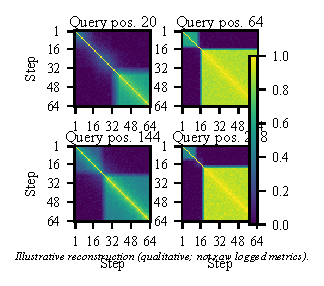
\includegraphics[width=\linewidth]{figures/attention_multi_position.pdf}
        \caption{Cross-step attention similarity for representative query positions.}
        \label{fig:cross_step_heatmap}
    \end{subfigure}
    \hfill
    \begin{subfigure}[b]{0.49\columnwidth}
        \centering
        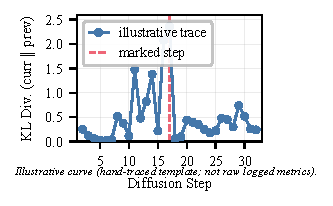
\includegraphics[width=\linewidth]{figures/attention_similarity_curve.pdf}
        \caption{KL divergence between consecutive denoising steps.}
        \label{fig:cross_step_curve}
    \end{subfigure}

    \caption{Attention patterns in DLMs are locally consistent but not globally stationary across denoising steps. (a) Cross-step similarity heatmaps show high similarity within nearby steps but clear discrepancies between distant ones. (b) KL divergence between consecutive steps reveals sharp spikes at transition points, indicating abrupt pattern shifts.}
    \label{fig:cross_step}
\end{figure}

Motivated by these two observations, we propose \textbf{Step-dLLM}, a sparse attention framework tailored for diffusion LLMs. Step-dLLM partitions the denoising trajectory into groups of consecutive steps. The first step in each group serves as an \emph{anchor step} that computes full attention and simultaneously extracts a block-sparse mask; the remaining steps reuse this mask with freshly computed queries, keys, and values, reducing per-step cost from $\mathcal{O}(L^2)$ to $\mathcal{O}(L \cdot k \cdot b)$. The mask is periodically refreshed, bounding its staleness and accommodating the evolving attention structure. Additionally, Step-dLLM allocates a global sparsity budget across heads in proportion to each head's cumulative saliency, allowing concentrated heads to be compressed aggressively while reserving capacity for dispersed yet important ones. Both components are realized through fused Triton kernels---a modified Flash Attention kernel that emits block-level saliency scores as a byproduct, and a block-sparse attention kernel that gathers only the selected key--value blocks---ensuring that the algorithmic gains translate into wall-clock speedups.

In summary, our contributions are as follows:
\begin{itemize}
    \item We present an empirical analysis of sparse attention in diffusion LLMs and identify two key properties: (i) the sparse attention pattern is locally consistent but not globally reusable across denoising steps, and (ii) different attention heads exhibit markedly different concentration behaviors. These findings expose fundamental limitations of one-shot mask reuse and uniform token-level sparsification employed by prior methods.

    \item We propose \textbf{Step-dLLM}, a sparse attention framework for diffusion LLMs that refreshes the sparse mask at selected anchor steps and allocates sparse computation globally across heads according to head-specific saliency, achieving a principled accuracy--efficiency trade-off.

    \item We design fused Triton kernels for both anchor-step mask extraction and non-anchor-step block-sparse attention, and conduct extensive experiments on representative diffusion LLMs, demonstrating that Step-dLLM achieves superior accuracy--efficiency trade-offs compared to prior sparse baselines, especially under high sparsity regimes.
\end{itemize}

\section{Background and Related Work}
\label{sec:background}

\subsection{Preliminaries: Discrete Diffusion Language Models}
\label{sec:prelim}

Discrete diffusion language models (dLLMs) generate text by iteratively unmasking a fully corrupted sequence over $S$ denoising steps. Let $\mathcal{V}$ denote the vocabulary and $L$ the total sequence length comprising $m$ prompt tokens and $L-m$ response tokens at positions $\mathcal{R}=\{m{+}1,\ldots,L\}$. Starting from $x^{(0)}$ in which all response positions are set to $[\mathrm{MASK}]$, each step $s$ applies a Transformer denoiser $f_\theta$ to produce per-token distributions $\pi_i^{(s)}=\mathrm{Softmax}(f_\theta(x^{(s)})_i)$ for $i\in\mathcal{R}$. A subset of currently masked positions is then unmasked by sampling from $\pi_i^{(s)}$ according to a decreasing mask-ratio schedule, while prompt tokens remain frozen throughout. After $S$ steps all masks are removed and $x^{(S)}$ is returned.

Crucially, because dLLMs predict \emph{all} masked tokens simultaneously at each step, $f_\theta$ employs \textbf{bidirectional} (non-causal) self-attention over the full length-$L$ sequence. This means every denoising step incurs $\mathcal{O}(L^2)$ attention cost and, unlike autoregressive models, cannot directly leverage KV caching. Reducing this per-step quadratic cost is the central goal of our work.

\subsection{Related Work}
\label{sec:related}

\paragraph{Diffusion language models.}
Extending diffusion to discrete tokens, D3PM~\citep{austin2021d3pm} introduced learnable transition matrices, SEDD~\citep{lou2024sedd} proposed score-entropy-based training, and MDLM~\citep{sahoo2024mdlm} showed that a simplified masked diffusion objective substantially closes the gap with autoregressive (AR) models. LLaDA~\citep{nie2025llada} scaled this paradigm to 8B parameters, rivaling LLaMA3 8B across diverse benchmarks, with subsequent extensions to multimodal~\citep{you2025lladav}, mixture-of-experts~\citep{llada-moe2025}, and preference-optimized variants~\citep{zhu2025llada15}.

\paragraph{Efficient inference for dLLMs.}
Efforts to accelerate diffusion language models follow two directions.
One line of work reduces the number of sampling steps by introducing block-wise autoregressive generation, which enables KV caching and inter-block parallelism~\citep{arriola2025block,llada2,wu2025fastdllm,d2f2025}.
The other line reduces per-step cost by exploiting the temporal redundancy of attention maps across denoising timesteps~\citep{yuan2024ditfastattn,zhang2025spargeattn,liteattention2025}; however, these methods are designed for continuous-domain diffusion transformers and do not transfer to the masked discrete setting, where attention patterns exhibit fundamentally different dynamics.

\paragraph{Sparse attention.}
Classical sparse attention mechanisms impose fixed patterns---strided, sliding-window, or global-token masks---to achieve sub-quadratic complexity~\citep{child2019sparse,beltagy2020longformer,zaheer2020bigbird}, but sacrifice adaptivity to input-dependent saliency.
A recent wave of dynamic methods instead constructs block-sparse masks on the fly, using strategies such as online index estimation, query-aware selection, or learned gating~\citep{jiang2024minference,tang2024quest,zhu2025tactic,gao2024seerattention,yuan2025nsa}.
Complementary kernel-level advances~\citep{dao2022flashattention,dao2023flashattention2,ye2025flashinfer,xu2025xattention} further reduce wall-clock time through IO-aware tiling and block-sparse execution.
Crucially, all of the above assume \emph{causal} attention and recompute the sparse mask at every forward pass.
Our work departs from this paradigm in two ways: we target the \emph{bidirectional} attention of dLLMs, and we \emph{amortize} mask computation across diffusion steps by leveraging the temporal stability of attention patterns unique to iterative denoising (Section~\ref{sec:mask_reuse}).
\section{Analysis and Motivations}
\label{sec:analysis}
In this section, we analyze the attention map behaviors during the generation time and illustrate how the observations motivate the adaptive attention sparse updates.

\subsection{Cross-step attention similarity}
Existing sparsity methods in DLM, such as SparseD \cite{wang2025sparsed}, are built on the observation that attention patterns exhibit noticeable temporal consistency across inference steps. Based on this observation, they estimate the sparse attention pattern once and reuse it in subsequent denoising steps, thereby avoiding repeated pattern construction overhead. While this assumption is partially valid, we find that it is insufficient to fully characterize attention dynamics in DLLMs. For a query position $i$ at denoising step $s$, we define its attention pattern as $\mathbf{a}_i^{(s)}=\mathrm{Softmax}\left(\frac{\mathbf{q}_i^{(s)}\mathbf{K}^{(s)\top}}{\sqrt{d}}\right)$, which represents the attention distribution of the query token over all key positions at step $s$.

Unlike autoregressive decoding, DLLM inference proceeds through an iterative denoising process, in which the visible context and token certainty evolve continuously across steps. As more tokens become unmasked, the dependency structure of the sequence is gradually refined, and the attention pattern may be reorganized accordingly. In particular, some key positions that are not salient at early steps can become pivotal at later steps.  As illustrated in Figure~\ref{fig:attention_pattern_across_steps}, which compares two groups of nearby denoising steps, the attention patterns are highly consistent within Steps 29--31 and within Steps 39--41, suggesting local reusability across nearby steps. However, comparing these two groups reveals a clear pattern shift: a new pivotal token at key position 95 emerges in Steps 39--41 but is not prominent in Steps 29--31. This indicates that, although the sparse attention pattern can be reused locally, it is not fully stationary throughout denoising.

As further shown in Figure~\ref{fig:cross_step_curve}, the change between two consecutive attention patterns is measured by the KL divergence $D_{\mathrm{KL}}\!\left(\mathbf{a}_i^{(s)} \,\|\, \mathbf{a}_i^{(s-1)}\right)=\sum_{j=1}^{L}\mathbf{a}_{i,j}^{(s)}\log\frac{\mathbf{a}_{i,j}^{(s)}}{\mathbf{a}_{i,j}^{(s-1)}}$. Although many neighboring steps remain relatively similar, there exist several transition steps where the divergence increases sharply, suggesting abrupt changes in the underlying attention structure. This implies that directly reusing a sparse pattern estimated at early steps may lead to stale sparsity decisions: newly important attention links can be missed, while computation is still spent on entries that are no longer critical. These observations motivate us to refresh the sparse attention matrix at some selected anchor steps.





% In DLLMs, the attention computation is formulated as$\mathrm{Out}=\mathrm{Softmax}\left(\frac{QK^\top}{\sqrt{d}}\right)V $, where the corresponding attention scores are defined as $\mathrm{AttnScore}=\mathrm{Softmax}\left(\frac{QK^\top}{\sqrt{d}}\right)$. Here, \(Q,K \in \mathbb{R}^{\mathrm{seq}\times d}\), and \(\mathrm{seq}\) denotes the total sequence length consisting of both the prompt and the generated context. Across all denoising steps, attention is computed over this full sequence. \zz{need polishing}

% for different position tokens, since DLLMs will update the token by unmasking step by step, some position will generate a token and we call this step i as the "tuning point" for the position x\_i. Before this step, this position behaves as decoding, trying to denoising and find the maximal logits and after this step, this position changes to prefilling, which can provide the information for the next steps of token generation.

% For example, referring to Figure 2, during the first two steps, the word tokens are denoised, and then performanced as the prefilling tokens in following steps.
% \xz{1. figure: cross-step similarity and non-similarity case - two figures? one figure?}


% To understand the attention behaviors cross steps, we first measure the attention score cosine similarity across steps. The measurement on the cosine similarity is presented in Figure xxx. Notably, the similarity between steps is \zz{}
% \red{here we need to have some data to present the across-step similarity regular pattern}

% \red{need to update the figure? heatmap}

\begin{figure}[h]
    \centering
    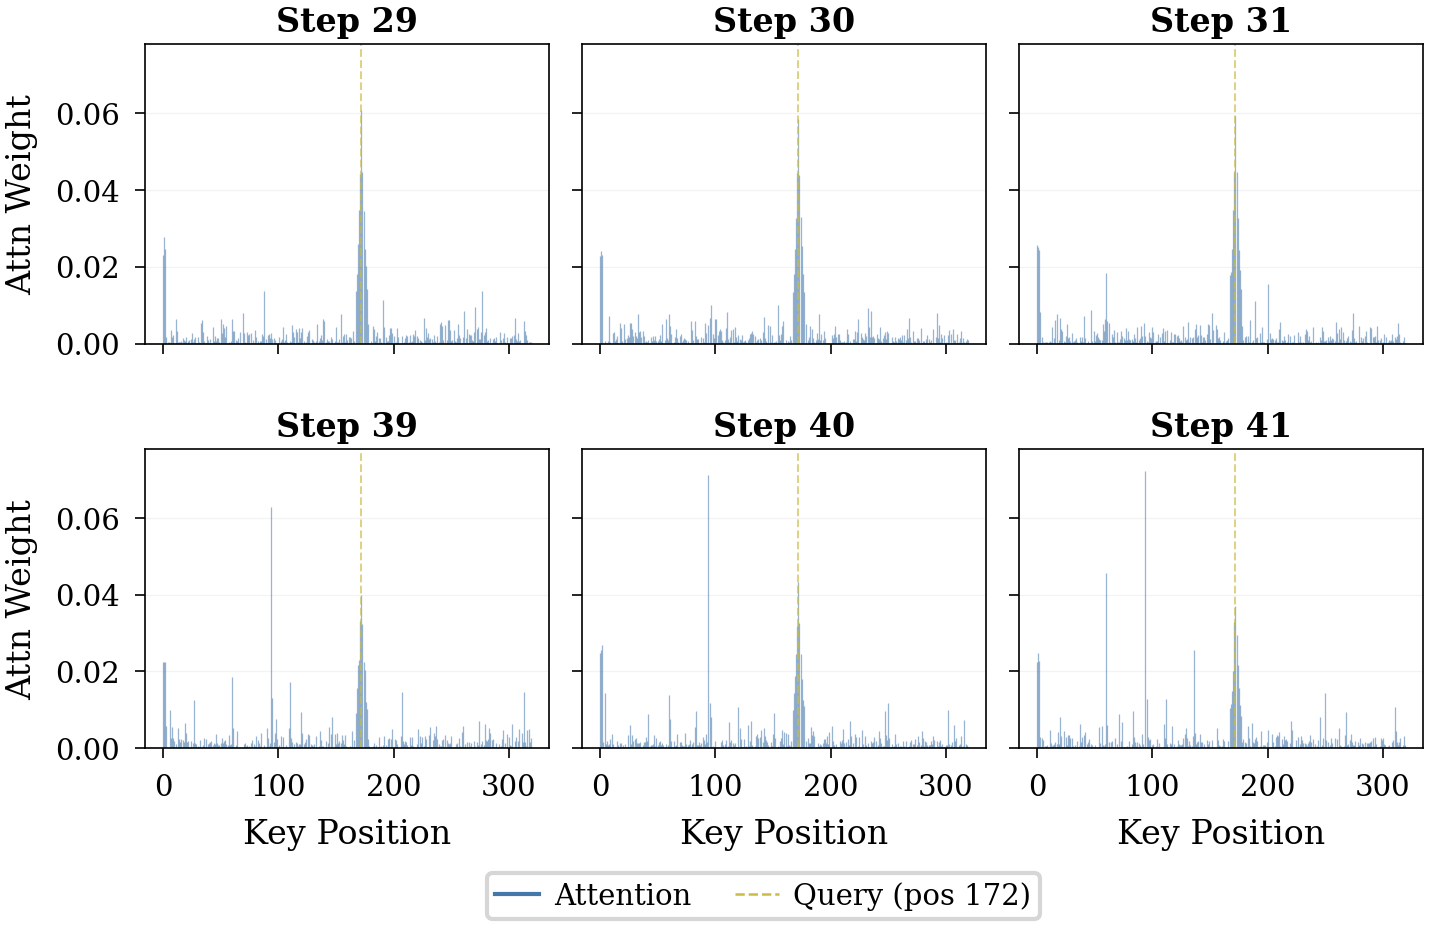
\includegraphics[width=1.0\linewidth]{figures/panels_6step_2x3.png}
    \caption{Attention patterns across different denoising steps.}
    \label{fig:attention_pattern_across_steps}
\end{figure}


\subsection{Head-wise Heterogeneity in Sparse Attention}

Recent sparse DLM methods reduce inference cost by exploiting sparsity during the denoising process. In particular, SparseD\cite{wang2025sparsed} performs sparse attention computation by selecting important token interactions according to token-level attention saliency, while Sparse-dLLM \cite{} improves efficiency through token-level cache eviction. These designs have shown promising efficiency gains in DLM inference. However, they also implicitly treat the token as the primary unit of sparsification, assuming that the importance of a token is largely consistent across attention heads.  We find that this assumption is overly coarse for DLMs.

As shown in Figure~\ref{fig: attention_heterogeneity}(a), even for the same query token, different attention heads can exhibit substantially different attention patterns. 
Some heads focus sharply on a small set of key positions, while others attend more broadly or emphasize entirely different regions. 
This indicates that head-specific behaviors are not merely a secondary effect, but a fundamental property of sparse attention in DLMs. 
Consequently, a unified token-level sparsity decision may be suboptimal: a token that is highly important for one head can be much less informative for another. 
Applying the same sparse mask or compression rule across all heads therefore risks preserving unnecessary computations in some heads while discarding critical attention scores in others.

Moreover, the heterogeneity across heads is reflected not only in attended positions, but also in the concentration of attention mass. 
Figure~\ref{fig: attention_heterogeneity}(b) visualizes the cumulative density of attention scores for different heads. 
We observe that the concentration behaviors vary markedly across heads: some heads are highly concentrated, where preserving only a small fraction of top-scoring entries already retains most of the attention mass, whereas other heads are much more dispersed and require a substantially larger fraction to achieve the same coverage. 
For example, certain heads can preserve around $90\%$ of the attention mass with only about $10\%$ of the entries, while others may require close to $50\%$. 
This suggests that different heads have different compression sensitivities and thus should not be assigned the same sparsity budget.

This observation is qualitatively different from prior token-level acceleration strategies in DLMs. 
SparseD emphasizes that sparse patterns are highly reusable across denoising steps and therefore pre-computes sparse patterns once and reuses them later, while Sparse-dLLM leverages the temporal stability of token saliency to evict low-importance cache entries. 
In contrast, our analysis highlights that, even when sparsity is exploited, the effective compression granularity should be head-aware rather than purely token-level. 
In other words, the key challenge is not only which tokens to preserve, but also how much computation budget each head should receive.

Motivated by this head-wise heterogeneity, we allocate the sparse attention budget globally across heads instead of enforcing a uniform token-level or per-head compression ratio. 
This design allows highly concentrated heads to be compressed more aggressively, while reserving more computation for heads with more dispersed yet important attention patterns. 
As a result, the sparse budget can be utilized more effectively, leading to a better trade-off between efficiency and model quality.


\begin{figure}[t]
    \centering
    \begin{subfigure}[b]{0.49\columnwidth}
        \centering
        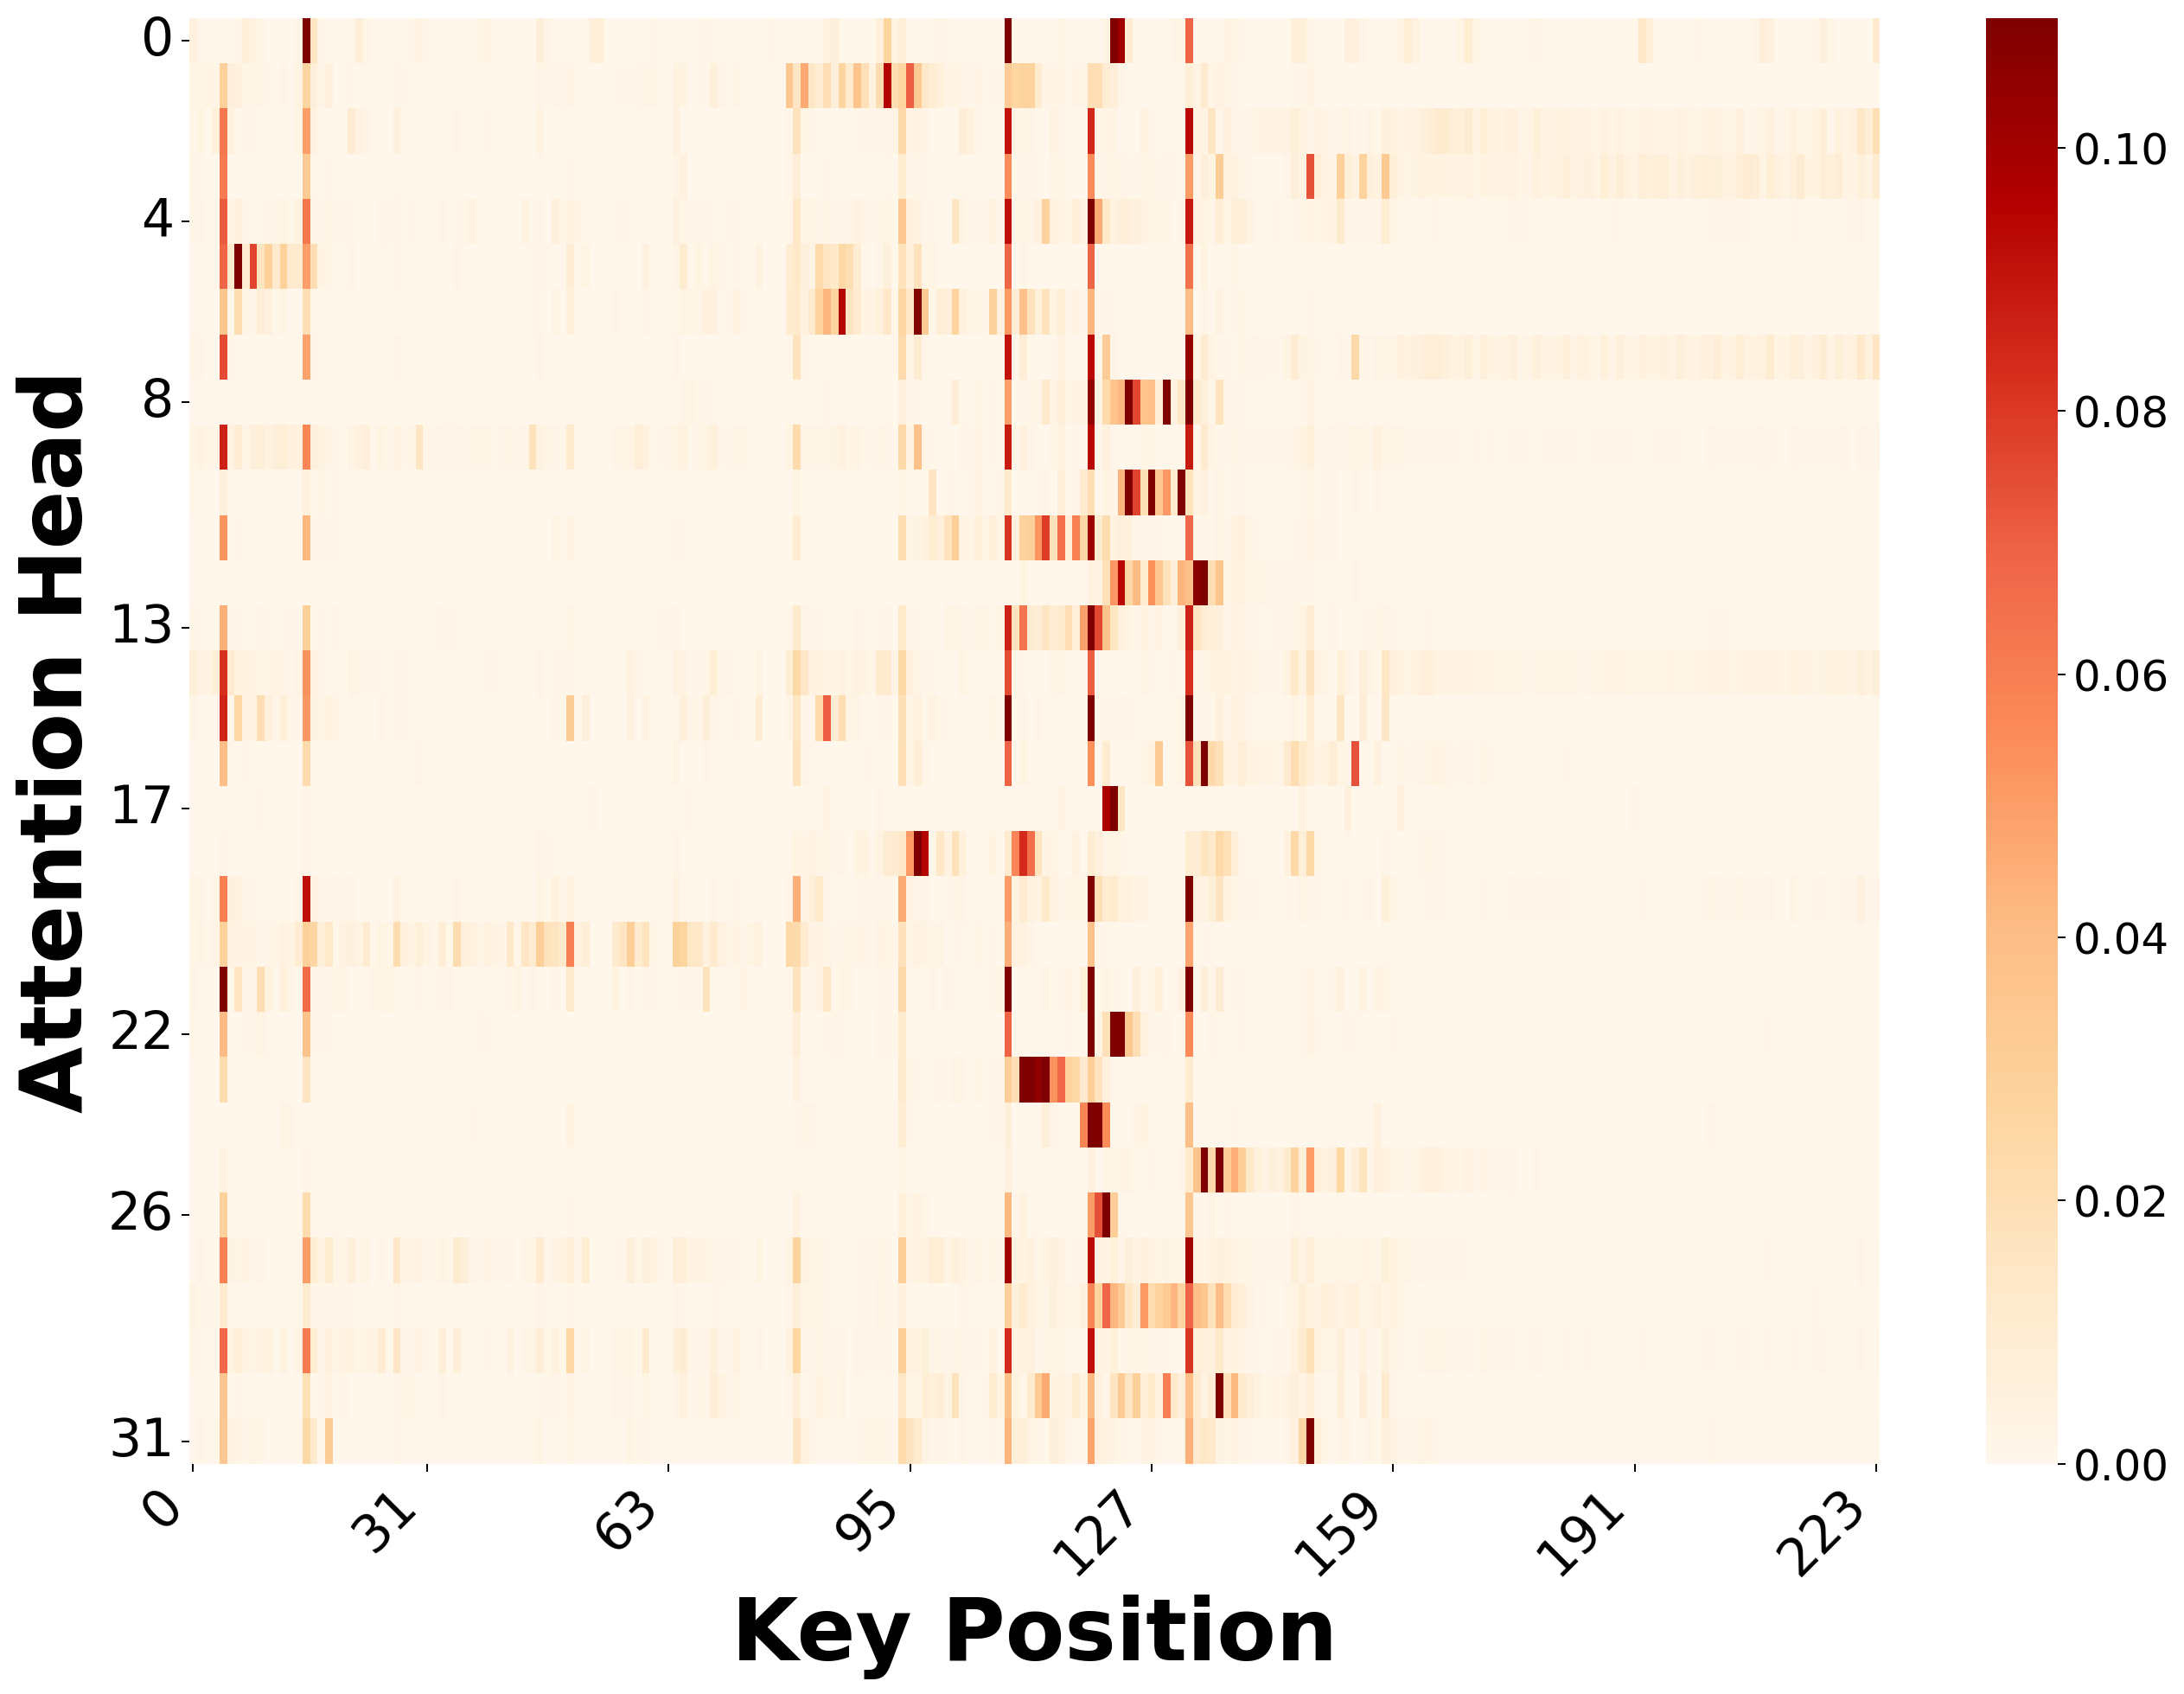
\includegraphics[width=\linewidth]{figures/difference_between_attention_heads.png}
        \caption{Attention patterns of different heads for the same query position, showing head-wise heterogeneity.}
    \end{subfigure}
    \hfill
    \begin{subfigure}[b]{0.49\columnwidth}
        \centering
        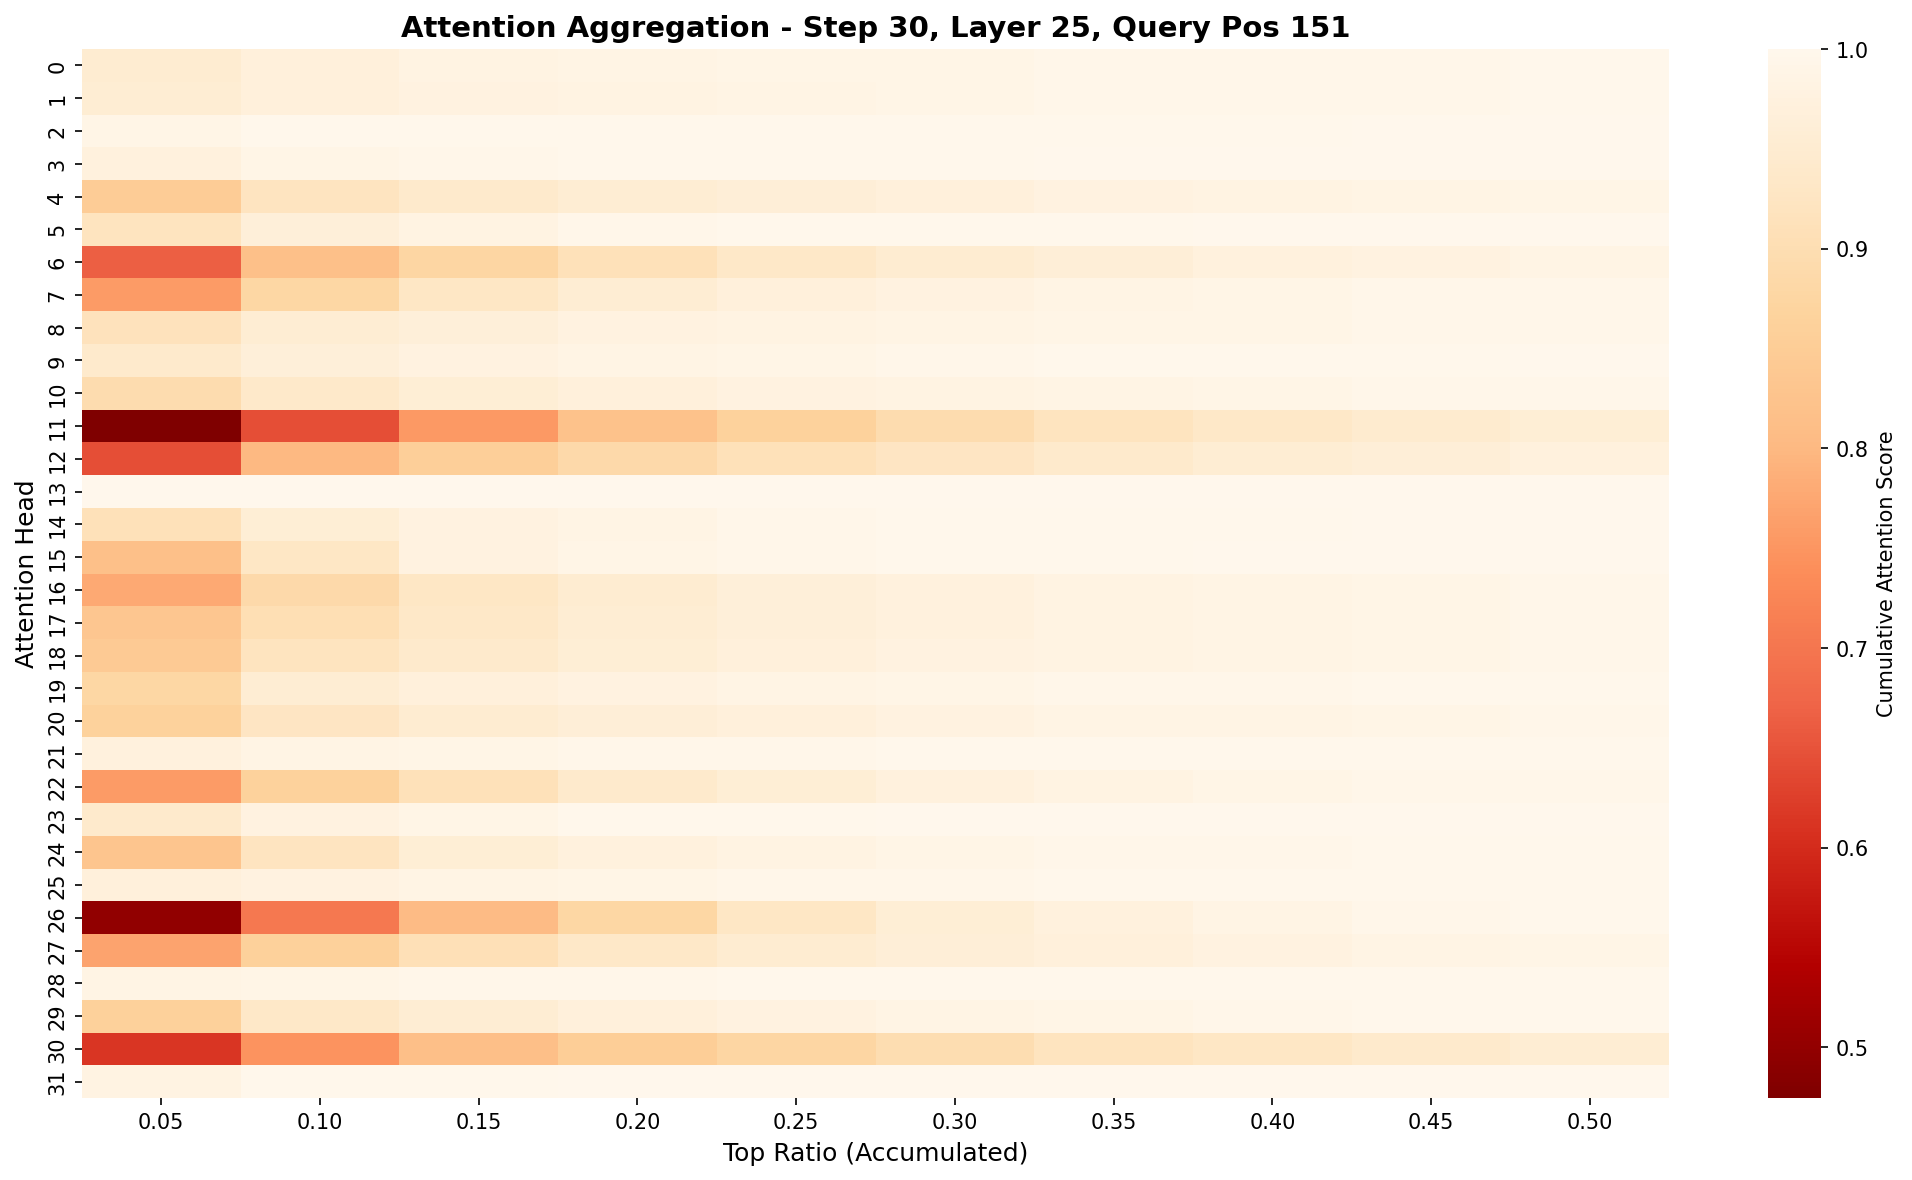
\includegraphics[width=\linewidth]{figures/attention_aggregation_step30_layer25_pos151.png}
        \caption{Cumulative attention mass across heads, illustrating varying concentration levels.}
        \label{fig:budget_cross_head}
    \end{subfigure}

    \caption{Head-wise heterogeneity in attention patterns. (a) Different heads attend to substantially different key positions for the same query. (b) Cumulative attention density varies markedly across heads, indicating different compression sensitivities.}
    \label{fig: attention_heterogeneity}
\end{figure}



% % Motivated by Section 3.2, we proposes a step-aware sparse mask update to reuse the similarity of sparse patterns.

% % Let s be the current diffusion step and L=l+c be the total sequence length. First, we do the attention in the 
% As demonstrated in Section~3.2, attention maps exhibit substantial similarity across consecutive diffusion steps. To exploit this temporal redundancy, we propose a cross-step attention reuse mechanism. Let $s$ denote the current diffusion step, $L$ the total sequence length, $b$ the block size, and $k$ the number of retained blocks per query block. We partition the $\mathbf{Q}, \mathbf{K}, \mathbf{V}$ matrices into blocks of size $b$, yielding $N_b = \lceil L/b \rceil$ blocks along the sequence dimension.

% \textbf{Anchor step computation.} At designated anchor step $i$, we compute full attention using a modified flash attention kernel that simultaneously produces both the attention output and a block-level sparsity mask. For each query block $p$ and key block $q$, we derive a coarse-grained saliency score via block-wise max-pooling over the attention logits:
% \begin{equation}
% \mathbf{M}_{pq} = \max_{(m,n) \in [b] \times [b]} \frac{(\mathbf{Q}_p)_m (\mathbf{K}_q)_n^\top}{\sqrt{d}}
% \end{equation}
% where $\mathbf{M} \in \mathbb{R}^{N_b \times N_b}$ captures the maximum attention affinity within each block pair. For each query block $p$, we retain only the top-$k$ most salient key blocks $\mathcal{I}_p = \mathrm{Top\text{-}k}\!\left(\{\mathbf{M}_{pq}\}_{q=1}^{N_b}\right)$, forming the sparse mask $\mathcal{I} = \{\mathcal{I}_p\}_{p=1}^{N_b}$. The full attention output is computed simultaneously within the fused kernel, so the anchor step jointly returns:
% \begin{equation}
% \mathcal{I},\ \mathbf{O}^{(i)} = \texttt{Modified-Flash-Attn}(\mathbf{Q}, \mathbf{K}, \mathbf{V},\ b,\ k)
% \end{equation}

% \textbf{Non-anchor step computation.} At subsequent steps $i{+}1, i{+}2, \ldots$, we reuse the cached mask indices $\mathcal{I}$ and perform block-sparse attention. For each query block $p$, attention is restricted to the selected key blocks:
% \begin{equation}
% \mathbf{O}^{(i+t)}_p = \mathrm{softmax}\!\left(\frac{\mathbf{Q}_p^{(i+t)} \left[\mathbf{K}_{q}^{(i+t)}\right]_{q \in \mathcal{I}_p}^\top}{\sqrt{d}}\right) \left[\mathbf{V}_{q}^{(i+t)}\right]_{q \in \mathcal{I}_p}
% \end{equation}
% where the superscript $(i{+}t)$ indicates that $\mathbf{Q}, \mathbf{K}, \mathbf{V}$ are freshly computed at step $i{+}t$, while only the sparsity pattern $\mathcal{I}$ is inherited from the anchor step. This reduces the per-step complexity from $\mathcal{O}(L^2)$ to $\mathcal{O}(L \cdot k \cdot b)$, amortizing the cost of full attention over multiple diffusion steps:
% \begin{equation}
% \mathbf{O}^{(i+t)} = \texttt{Block-Sparse-Attn}(\mathbf{Q}^{(i+t)}, \mathbf{K}^{(i+t)}, \mathbf{V}^{(i+t)},\ \mathcal{I})
% \end{equation}

% \textbf{Adaptive re-anchoring.} The sparsity pattern $\mathcal{I}$ derived at an anchor step is not perpetually valid: as illustrated in Figure~\ref{fig:cross_step}, the attention score distribution evolves non-monotonically across diffusion steps, exhibiting pronounced transition points as generation progresses from early denoising to final convergence. Reusing a stale mask beyond these transitions degrades output quality. To balance computational savings against mask fidelity, we introduce a periodic re-anchoring schedule governed by a refresh interval $\Delta$. Every $\Delta$ steps, we designate the current step as a new anchor, recompute full attention via the modified Flash Attention kernel, and refresh the cached mask $\mathcal{I}$. Between consecutive anchors, the mask is frozen and block-sparse attention is applied. The overall procedure, summarized in Algorithm~\ref{alg:step_aware_sparse}, thus amortizes the $\mathcal{O}(L^2)$ cost of full attention over $\Delta$ steps, yielding an average per-step complexity of $\mathcal{O}\!\left(\frac{L^2}{\Delta} + L \cdot k \cdot b\right)$, which approaches $\mathcal{O}(L \cdot k \cdot b)$ for moderate $\Delta$.

% \begin{algorithm}[t]
% \caption{Step-Aware Sparse Attention with Periodic Re-Anchoring}
% \label{alg:step_aware_sparse}
% \begin{algorithmic}[1]
% \Require Diffusion steps $S$, block size $b$, top-$k$ budget, re-anchor interval $\Delta$
% \Ensure Output sequence $\mathbf{O}^{(s)}$ for each step $s = 1, \ldots, S$
% \State $\mathcal{I} \gets \varnothing$ \Comment{Initialize cached sparse mask}
% \For{$s = 1$ \textbf{to} $S$}
%     \State Compute $\mathbf{Q}^{(s)}, \mathbf{K}^{(s)}, \mathbf{V}^{(s)}$ from the current hidden states
%     \If{$s \equiv 1 \pmod{\Delta}$} \Comment{Anchor step}
%         \State $\mathcal{I},\; \mathbf{O}^{(s)} \gets \texttt{Modified-Flash-Attn}\!\left(\mathbf{Q}^{(s)}, \mathbf{K}^{(s)}, \mathbf{V}^{(s)},\; b,\; k\right)$
%         \State \Comment{Full attention + mask extraction}
%     \Else \Comment{Non-anchor step}
%         \State $\mathbf{O}^{(s)} \gets \texttt{Block-Sparse-Attn}\!\left(\mathbf{Q}^{(s)}, \mathbf{K}^{(s)}, \mathbf{V}^{(s)},\; \mathcal{I}\right)$
%         \State \Comment{Sparse attention with cached mask}
%     \EndIf
% \EndFor
% \end{algorithmic}
% \end{algorithm}


% \paragraph{Head-adaptive sparsity budget.}
% Different attention heads in diffusion language models capture distinct structural patterns---some heads attend broadly across the sequence while others focus locally. Imposing a uniform per-head sparsity budget (e.g., a fixed sliding-window size) fails to accommodate this heterogeneity. Instead, we allocate a global sparsity budget across all heads and let each head claim capacity according to its attention saliency. Concretely, let $H$ denote the number of attention heads and $k_h$ the number of retained blocks for head $h$. We constrain the total budget as:
% \begin{equation}
% \sum_{h=1}^{H} k_h = K_{\text{total}}, \quad k_h \geq k_{\min},
% \label{eq:budget}
% \end{equation}
% where $K_{\text{total}}$ is the aggregate block budget across all heads and $k_{\min}$ is a minimum allocation that guarantees each head retains at least a baseline level of context. At each anchor step, we rank heads by their cumulative block-level saliency scores $\sum_{p,q} \mathbf{M}^{(h)}_{pq}$ and distribute the remaining budget $K_{\text{total}} - H \cdot k_{\min}$ proportionally to heads with higher total saliency, allowing attention-heavy heads to retain more key blocks while pruning redundant ones aggressively.

% \paragraph{Customized Triton kernels.}
% To realize the above scheme efficiently on GPU, we implement two fused Triton kernels. The \texttt{Modified-Flash-Attn} kernel extends standard Flash Attention~\citep{dao2022flashattention} to emit the block-level saliency matrix $\mathbf{M}$ as a byproduct of the forward pass, producing both the full attention output $\mathbf{O}$ and the sparse mask $\mathcal{I}$ in a single kernel launch without redundant recomputation of the attention logits. The \texttt{Block-Sparse-Attn} kernel consumes the cached mask indices $\mathcal{I}$ and performs gather-based block-sparse matrix multiplication, loading only the selected key--value blocks into shared memory. Together, the two kernels eliminate the need for any materialized $L \times L$ attention matrix, keeping peak memory at $\mathcal{O}(L \cdot k \cdot b)$ throughout both anchor and non-anchor steps.

\section{Methodology}
\label{sec:method}

We present \textbf{Step-dLLM}, an efficient inference framework for diffusion language models. The key observation (Section~\ref{sec:analysis}) is that attention maps change slowly across consecutive diffusion steps, yet vary at different rates throughout the generation process. Step-dLLM exploits this structure through three integrated components: (i)~a \emph{cross-step mask reuse} scheme that amortizes the cost of identifying sparse patterns (Section~\ref{sec:mask_reuse}), (ii)~a \emph{head-adaptive budget} that allocates sparsity non-uniformly across attention heads (Section~\ref{sec:mask_construction}), and (iii)~\emph{fused Triton kernels} that make both anchor and non-anchor steps hardware-efficient (Section~\ref{sec:kernels}). Figure~\ref{fig:step_dllm_overview} provides an overview.

\begin{figure}[t]
    \centering
    \includegraphics[width=0.95\linewidth]{figures/StepdLLM.png}
    \caption{Overview of \textbf{Step-dLLM}. Anchor steps compute full attention and extract a block-sparse mask via a fused kernel. Non-anchor steps reuse the cached mask with fresh $\mathbf{Q}, \mathbf{K}, \mathbf{V}$, reducing per-step cost from $\mathcal{O}(L^2)$ to $\mathcal{O}(L \cdot k \cdot b)$. The mask is periodically refreshed every $\Delta$ steps.}
    \label{fig:step_dllm_overview}
\end{figure}

%% ----------------------------------------------------------------
\subsection{Cross-Step Sparse Mask Reuse}
\label{sec:mask_reuse}

The per-step $\mathcal{O}(L^2)$ cost of full bidirectional attention is the dominant bottleneck in dLLM inference. Our key observation (Section~\ref{sec:analysis}) is that, although the attention maps evolve across diffusion steps, adjacent steps share highly similar block-level sparsity structures (Figure~\ref{fig:cross_step}). This motivates a simple strategy: \emph{compute the sparse mask once, then reuse it for several subsequent steps}, amortizing the cost of mask identification over a group of steps.

Formally, let $b$ denote the block size and $N_b = \lceil L/b \rceil$ the number of blocks. We partition the $S$ diffusion steps into consecutive groups of size $\Delta$. Within each group, the first step serves as the \emph{anchor} and the remaining $\Delta{-}1$ steps reuse the anchor's mask.

\paragraph{Anchor steps} compute full attention and simultaneously extract a block-level sparsity mask $\mathcal{I}$ (construction detailed in Section~\ref{sec:mask_construction}), both produced by a single fused kernel launch with no redundant recomputation:
\begin{equation}
    \mathcal{I},\ \mathbf{O}^{(s)} = \texttt{Modified-Flash-Attn}(\mathbf{Q}^{(s)}, \mathbf{K}^{(s)}, \mathbf{V}^{(s)},\ b).
\end{equation}

\paragraph{Non-anchor steps} freeze the cached mask $\mathcal{I}$ and restrict attention to the selected blocks. Note that only the sparsity \emph{pattern} is inherited---the queries, keys, and values are freshly computed from the current step's hidden states, so the attention \emph{weights} remain faithful to the evolving token representations:
\begin{equation}
    \mathbf{O}^{(s)} = \texttt{Block-Sparse-Attn}(\mathbf{Q}^{(s)}, \mathbf{K}^{(s)}, \mathbf{V}^{(s)},\ \mathcal{I}).
\end{equation}

The mask is refreshed every $\Delta$ steps, bounding the staleness of $\mathcal{I}$ and accommodating the non-stationary nature of the attention distribution. This yields an average per-step complexity of $\mathcal{O}\!\bigl(\frac{L^2}{\Delta} + L \cdot k \cdot b\bigr)$, which approaches $\mathcal{O}(L \cdot k \cdot b)$ for moderate $\Delta$. The complete procedure is summarized in Algorithm~\ref{alg:step_aware_sparse}.

\begin{algorithm}[t]
\caption{Step-dLLM Inference}
\label{alg:step_aware_sparse}
\begin{algorithmic}[1]
\Require Diffusion steps $S$, block size $b$, global budget $K_{\text{total}}$, per-head minimum $k_{\min}$, re-anchor interval $\Delta$, number of heads $H$
\Ensure Output $\mathbf{O}^{(s)}$ for each step $s = 1, \ldots, S$
\State $\mathcal{I} \gets \varnothing$ \Comment{Cached block-sparse mask across all heads}
\For{$s = 1$ \textbf{to} $S$}
    \State Compute $\mathbf{Q}^{(s)}, \mathbf{K}^{(s)}, \mathbf{V}^{(s)} \in \mathbb{R}^{H \times L \times d}$ from current hidden states
    \If{$\mathcal{I} = \varnothing$ \textbf{or} $s \equiv 1 \pmod{\Delta}$} \Comment{Anchor step}
        \State $\mathbf{M},\; \mathbf{O}^{(s)} \gets \texttt{Modified-Flash-Attn}\!\left(\mathbf{Q}^{(s)}, \mathbf{K}^{(s)}, \mathbf{V}^{(s)},\; b\right)$
            \Comment{$\mathbf{M} \in \mathbb{R}^{H \times N_b \times N_b}$, all heads in parallel}
        \State $S_h \gets \sum_{p,q} \mathbf{M}^{(h)}_{pq}$ for $h = 1, \ldots, H$
            \Comment{Per-head cumulative saliency}
        \State Allocate $\{k_h\}_{h=1}^{H}$ from $K_{\text{total}}$ proportionally to $\{S_h\}$ subject to $k_h \geq k_{\min}$ \Comment{Eq.~\eqref{eq:budget}}
        \State $\mathcal{I}^{(h)}_p \gets \mathrm{Top\text{-}k_h}\!\left(\{\mathbf{M}^{(h)}_{pq}\}_{q=1}^{N_b}\right)$ for all $h, p$
            \Comment{Extract sparse mask}
    \Else \Comment{Non-anchor step}
        \State $\mathbf{O}^{(s)} \gets \texttt{Block-Sparse-Attn}\!\left(\mathbf{Q}^{(s)}, \mathbf{K}^{(s)}, \mathbf{V}^{(s)},\; \mathcal{I}\right)$
            \Comment{All heads in parallel, mask $\mathcal{I}$ reused}
    \EndIf
\EndFor
\end{algorithmic}
\end{algorithm}

%% ----------------------------------------------------------------
\subsection{Block-Sparse Mask Construction with Head-Adaptive Budget}
\label{sec:mask_construction}
%% ----------------------------------------------------------------

We now describe how the sparsity mask $\mathcal{I}$ is constructed at each anchor step. The procedure involves two stages: computing block-level saliency scores and allocating a non-uniform budget across heads.

\paragraph{Block-level saliency scoring.}
Let $L$ denote the total sequence length and $b$ the block size. We partition $\mathbf{Q}, \mathbf{K}, \mathbf{V}$ into $N_b = \lceil L/b \rceil$ blocks along the sequence dimension. For each attention head $h$, query block $p$, and key block $q$, we compute a coarse saliency score via block-wise max-pooling over the attention logits:
\begin{equation}
    \mathbf{M}^{(h)}_{pq} = \max_{(m,n) \in [b] \times [b]} \frac{(\mathbf{Q}^{(h)}_p)_m (\mathbf{K}^{(h)}_q)_n^\top}{\sqrt{d}},
\end{equation}
where $\mathbf{M}^{(h)} \in \mathbb{R}^{N_b \times N_b}$ captures the maximum attention affinity within each block pair for head $h$. This scoring is performed as a byproduct of the full attention computation inside the fused \texttt{Modified-Flash-Attn} kernel (Section~\ref{sec:kernels}), incurring no additional pass over the data.

\paragraph{Head-adaptive budget allocation.}
Different heads serve distinct structural roles: some attend globally across the full sequence while others focus on narrow local windows. Assigning a uniform block budget $k$ to every head either wastes capacity on locally-focused heads or starves globally-attending ones. We therefore impose a global budget shared across all $H$ heads:
\begin{equation}
    \sum_{h=1}^{H} k_h = K_{\text{total}}, \quad k_h \geq k_{\min},
    \label{eq:budget}
\end{equation}
where $K_{\text{total}}$ controls the overall computation--quality trade-off and $k_{\min}$ ensures every head retains a minimum context window. The surplus budget $K_{\text{total}} - H \cdot k_{\min}$ is distributed proportionally to each head's cumulative saliency $S_h = \sum_{p,q} \mathbf{M}^{(h)}_{pq}$, allowing attention-heavy heads to retain more key blocks while aggressively pruning redundant ones. Given the per-head budget $k_h$, the mask for head $h$ is:
\begin{equation}
    \mathcal{I}^{(h)}_p = \mathrm{Top\text{-}k_h}\!\left(\{\mathbf{M}^{(h)}_{pq}\}_{q=1}^{N_b}\right), \quad \mathcal{I}^{(h)} = \{\mathcal{I}^{(h)}_p\}_{p=1}^{N_b}.
\end{equation}
This formulation keeps the total computational envelope fixed at $K_{\text{total}}$ blocks while letting the distribution adapt to each head's functional demands.

\subsection{Fused Triton Kernel Implementation}
\label{sec:kernels}

The algorithmic gains described above are only realized if the underlying kernels can efficiently execute both full and sparse attention without materializing the $L \times L$ attention matrix. We implement two complementary fused kernels in Triton~\citep{tillet2019triton}. The first, \texttt{Modified-Flash-Attn}, extends Flash Attention~\citep{dao2022flashattention} to emit the block-level saliency matrix $\mathbf{M}^{(h)}$ as a byproduct of the forward pass: as the kernel tiles over key blocks in its inner loop, it maintains a running per-block maximum of the attention logits at negligible additional cost, so that a single kernel launch produces both the full attention output $\mathbf{O}$ and all saliency scores needed for mask construction without any redundant recomputation. The second, \texttt{Block-Sparse-Attn}, consumes the cached mask indices $\mathcal{I}^{(h)}$ and performs gather-based block-sparse attention---for each query block $p$, only the $k_h$ key--value blocks indicated by $\mathcal{I}^{(h)}_p$ are loaded into shared memory while all unselected blocks are skipped entirely, yielding wall-clock speedups proportional to the sparsity ratio $k_h / N_b$. Together, the two kernels keep peak memory at $\mathcal{O}(L \cdot k \cdot b)$ throughout both anchor and non-anchor steps.
\section{Experiments}

\subsection{Experimental Setup}
\textbf{Models and Benchmarks} We implement our method on two representative dLLMs, Llada-1.5 and Dream-7B-Instuct, to evaluate its effectiveness in accelerating the inference process across various tasks. We conduct experiments on four standard benchmarks covering diverse task types to ensure the broad applicability of our approach, including GSM8K (mathematical reasoning), MATH(mathematical problem solving), HumanEval (code generation), and Ruler (long context capability).   

\textbf{Baselines and Metrics}
To validate the effectiveness of our method, we compare Step-dLLM against several state-of-the-art dLLM-based approaches, including vanilla LLaDA and Dream, the sparse acceleration method for autoregressive models StreamingLLM, and training-free efficient dLLM methods such as Fast-dLLM and SparseD. We evaluate inference acceleration and generation quality using quantitative metrics. Inference speed is quantified by the wall-clock time required to complete each task under a fixed generation length, while generation quality is assessed using task-specific metrics, such as accuracy on GSM8K, to reflect model performance under different acceleration strategies.

\textbf{Implemention Details}
During inference, we use a single NVIDIA H100 GPU and fix the batch size to 1 for all models. In our proposed method Step-dLLM, we largely follow the hyperparameter settings of SparseD. Specifically, for all datasets, we set the granularity of sparsity computation (block size) to \(S = 16\) and the block length to \(L = 32\), which controls the proportion between autoregressive steps and diffusion steps. In addition, we set the refresh frequency of the attention mask matrix to 0.2, i.e., we update the global attention mask every \(0.2 \times N_{\text{steps}}\) denoising steps. For short-text datasets such as GSM8K and HumanEval, we set the sparsity budget to \(\rho = 50\%\), whereas for the long context dataset Ruler, we adopt a more conservative budget of \(\rho = 20\%\). We use the same configuration \((S, L, \rho)\) for SparseD. Regarding the parameter in SparseD that controls the use of full attention instead of sparse attention in the early steps, we set the proportion to \(\text{skip}\% = 5\%\). To ensure a fair comparison, we configure Fast-dLLM with the same block length \(L = 32\) and set the threshold to \(\text{threshold} = 0.9\). For StreamingLLM, we fix the proportion of sink tokens \(s_0\) to 10\% of the total generation length, and derive the sliding window size \(W\) from the sparsity budget as $W = (\rho - s_0) \cdot L_{\text{total}}.$
Across all methods, we set the total generation length \(L_{\text{total}}\) to be equal to the number of diffusion steps \(N_{\text{steps}}\). Additional details about the models, datasets, and baseline methods are provided in the Appendix.

\subsection{Main Results}

Tables~\ref{tab:main-bs16-llada} and~\ref{tab:main-bs16-dream} summarize the main comparison on LLaDA-1.5 and Dream-7B-Instruct. Overall, Step-dLLM provides the best accuracy--sparsity trade-off among sparse methods on both short-form and long-context benchmarks, and the advantage becomes more visible as sparsity increases.

On reasoning and code generation tasks, Step-dLLM stays close to dense decoding at moderate sparsity and degrades more gracefully than SparseD in the high-sparsity regime. At 50\% sparsity, its accuracy is already comparable to the dense baseline on both backbones. The difference becomes clearer at 90\% sparsity: on GSM8K, Step-dLLM improves over SparseD by 5.6 points on LLaDA-1.5 (35.25\% vs.\ 29.64\%) and by 10.5 points on Dream-7B-Instruct (32.68\% vs.\ 22.21\%). At 95\% sparsity, the gap further widens on GSM8K, where Step-dLLM retains 17.13\% and 15.31\% accuracy on the two models, compared with 9.86\% and 4.40\% for SparseD. Similar trends hold on MATH and HumanEval. This behavior is consistent with our core hypothesis: once denoising progresses, a mask computed only once becomes increasingly stale, while periodic refresh better matches the evolving attention structure.

The gains are even larger on long-context retrieval benchmarks. On NIAH and RULER, Step-dLLM remains much closer to dense performance on the harder multi-needle and compositional subtasks, where missing a small set of relevant positions can lead to a disproportionate accuracy drop. For example, on LLaDA-1.5 at 80\% sparsity, SparseD drops to 71.20\% on NIAH-S\_3 and 74.20\% on MK\_3, whereas Step-dLLM maintains 100.00\% and 99.60\%, respectively. A similar trend appears on Dream-7B-Instruct, where Step-dLLM improves over SparseD by 21.8 points on S\_3 and 18.6 points on MK\_3 at the same sparsity level. On RULER, Step-dLLM also yields clear gains on compositional tasks such as CWE, improving LLaDA-1.5 from 34.56\% to 54.16\% at 90\% sparsity. These results suggest that long-context generation is especially sensitive to stale sparse patterns, because the set of salient key positions can shift substantially across denoising steps.

In contrast, StreamingLLM performs poorly throughout and often collapses at high sparsity. On LLaDA-1.5, GSM8K drops from 74.07\% at 50\% sparsity to 19.11\% at 80\% sparsity and essentially zero at 90\%; Dream-7B-Instruct shows the same failure mode. This result is expected: StreamingLLM is designed for autoregressive causal attention, whereas diffusion LLMs rely on bidirectional interactions that evolve during denoising. The comparison therefore highlights that sparse patterns tailored for autoregressive decoding do not transfer directly to the diffusion setting.

\begin{table}[t]
\centering
\caption{Main results on LLaDA-1.5 with block size 16. All values are accuracy (\%). \textbf{Bold} marks the best result per sparsity level (excluding Dense).}
\label{tab:main-bs16-llada}
\setlength{\tabcolsep}{3.5pt}
\renewcommand{\arraystretch}{1.15}

\resizebox{\textwidth}{!}{%
\begin{tabular}{@{}ll ccc ccccccccc ccccc@{}}
\toprule
\multirow{2.5}{*}{\textbf{Method}} & \multirow{2.5}{*}{\textbf{Sparsity}}
  & \multicolumn{3}{c}{\textbf{Short-form}}
  & \multicolumn{8}{c}{\textbf{NIAH}}
  & \multicolumn{5}{c}{\textbf{RULER}} \\
\cmidrule(lr){3-5} \cmidrule(lr){6-13} \cmidrule(l){14-18}
& & GSM8K & Math & HumanE
  & $\text{S}_1$ & $\text{S}_2$ & $\text{S}_3$
  & $\text{MK}_1$ & $\text{MK}_2$ & $\text{MK}_3$
  & MQ & MV
  & VT & CWE & FWE & QS & QH \\
\midrule

Dense & --
  & \textbf{81.04} & \textbf{37.20} & \textbf{40.24}
  & \textbf{100.0} & \textbf{100.0} & \textbf{100.0} & \textbf{100.0}
  & \textbf{100.0} & \textbf{100.0} & \textbf{100.0} & \textbf{100.0}
  & \textbf{100.0} & \textbf{52.40} & \textbf{64.20} & \textbf{91.30} & \textbf{76.00} \\

\midrule
\multirow{3}{*}{StreamingLLM}
  & 50\% & 74.07 & \textbf{38.20} & 39.02
    & 20.80 & 20.20 & 18.40 & 21.20 & 20.40 & 15.40 & 19.20 & 14.40
    & 30.60 & 13.40 & 73.80 & 81.65 & 44.40 \\
  & 80\% & 19.11 & 13.60 & 19.51
    & 5.00 & 2.40 & 1.40 & 3.40 & 3.60 & 0.00 & 2.10 & 2.10
    & 6.56 & 3.02 & 76.27 & 20.48 & 22.40 \\
  & 90\% & 0.08 & 0.00 & 2.43
    & 0.00 & 0.00 & 0.00 & 0.00 & 0.00 & 0.00 & 0.00 & 0.00
    & 0.00 & 2.12 & 0.00 & 0.27 & 0.00 \\

\midrule
\multirow{4}{*}{SparseD}
  & 50\% & 80.59 & 37.40 & 42.68
    & \textbf{100.0} & \textbf{100.0} & \textbf{100.0} & \textbf{100.0}
    & \textbf{100.0} & \textbf{100.0} & \textbf{100.0} & \textbf{100.0}
    & \textbf{99.88} & 52.26 & \textbf{61.40} & \textbf{83.17} & 77.60 \\
  & 80\% & 53.68 & \textbf{28.20} & 36.59
    & \textbf{100.0} & \textbf{100.0} & 71.20 & \textbf{100.0}
    & \textbf{100.0} & 74.20 & 85.85 & 79.10
    & 94.28 & \textbf{57.80} & 45.40 & 83.48 & 77.80 \\
  & 90\% & 29.64 & 20.00 & 30.49
    & \textbf{100.0} & \textbf{100.0} & 76.60 & \textbf{100.0}
    & 99.80 & 77.20 & 82.85 & 80.60
    & 93.32 & 34.56 & 42.07 & 83.13 & 76.00 \\
  & 95\% & 9.86 & 9.40 & 20.12
    & \textbf{100.0} & \textbf{100.0} & 79.40 & \textbf{100.0}
    & \textbf{100.0} & 78.20 & 81.80 & 81.10
    & 86.64 & 39.92 & 39.00 & \textbf{81.97} & \textbf{73.60} \\

\midrule
\multirow{4}{*}{\textbf{Step-dLLM}}
  & 50\% & \textbf{82.71} & 36.80 & \textbf{42.68}
    & \textbf{100.0} & \textbf{100.0} & \textbf{100.0} & \textbf{100.0}
    & \textbf{100.0} & \textbf{100.0} & \textbf{100.0} & \textbf{100.0}
    & 99.60 & \textbf{53.16} & 60.87 & 83.03 & \textbf{78.60} \\
  & 80\% & \textbf{58.38} & 27.60 & \textbf{37.20}
    & \textbf{100.0} & \textbf{100.0} & \textbf{100.0} & \textbf{100.0}
    & 99.80 & \textbf{99.60} & \textbf{99.90} & \textbf{98.60}
    & \textbf{98.52} & 56.46 & \textbf{51.73} & \textbf{83.73} & \textbf{78.20} \\
  & 90\% & \textbf{35.25} & \textbf{21.60} & \textbf{32.93}
    & \textbf{100.0} & \textbf{100.0} & \textbf{100.0} & \textbf{100.0}
    & \textbf{100.0} & \textbf{97.60} & \textbf{99.65} & \textbf{95.90}
    & \textbf{94.00} & \textbf{54.16} & \textbf{46.80} & \textbf{83.48} & \textbf{76.40} \\
  & 95\% & \textbf{17.13} & \textbf{13.80} & \textbf{21.34}
    & \textbf{100.0} & \textbf{100.0} & \textbf{98.80} & \textbf{100.0}
    & \textbf{100.0} & \textbf{88.40} & \textbf{95.25} & \textbf{92.30}
    & \textbf{92.32} & \textbf{44.76} & \textbf{44.07} & 81.37 & 71.40 \\
\bottomrule
\end{tabular}%
}
\end{table}

\begin{table}[t]
\centering
\caption{Main results on Dream-7B-Instruct with block size 16. All values are accuracy (\%). \textbf{Bold} marks the best result per sparsity level (excluding Dense).}
\label{tab:main-bs16-dream}
\setlength{\tabcolsep}{3.5pt}
\renewcommand{\arraystretch}{1.15}

\resizebox{\textwidth}{!}{%
\begin{tabular}{@{}ll ccc ccccccccc ccccc@{}}
\toprule
\multirow{2.5}{*}{\textbf{Method}} & \multirow{2.5}{*}{\textbf{Sparsity}}
  & \multicolumn{3}{c}{\textbf{Short-form}}
  & \multicolumn{8}{c}{\textbf{NIAH}}
  & \multicolumn{5}{c}{\textbf{RULER}} \\
\cmidrule(lr){3-5} \cmidrule(lr){6-13} \cmidrule(l){14-18}
& & GSM8K & Math & HumanE
  & $\text{S}_1$ & $\text{S}_2$ & $\text{S}_3$
  & $\text{MK}_1$ & $\text{MK}_2$ & $\text{MK}_3$
  & MQ & MV
  & VT & CWE & FWE & QS & QH \\
\midrule

Dense & --
  & \textbf{77.41} & \textbf{45.60} & --
  & \textbf{100.0} & \textbf{100.0} & \textbf{91.00} & \textbf{98.00}
  & \textbf{99.80} & \textbf{77.60} & \textbf{97.70} & \textbf{96.40}
  & \textbf{96.32} & \textbf{87.28} & \textbf{79.47} & \textbf{79.57} & \textbf{64.00} \\

\midrule
\multirow{3}{*}{StreamingLLM}
  & 50\% & 38.13 & 8.80 & 42.70
    & 10.00 & 11.00 & 9.00 & 11.00 & 8.80 & 12.40 & 8.75 & 10.30
    & 13.40 & 43.34 & 37.73 & \textbf{81.40} & 33.00 \\
  & 80\% & 19.56 & 10.40 & 25.00
    & 1.80 & 2.80 & 1.40 & 3.20 & 1.20 & 0.00 & 1.95 & 2.40
    & 0.36 & 4.54 & 4.33 & 19.18 & 19.60 \\
  & 90\% & 0.00 & 0.00 & 2.44
    & 0.00 & 0.00 & 0.00 & 0.00 & 0.00 & 0.00 & 0.00 & 0.00
    & 0.00 & 0.00 & 0.00 & 0.00 & 0.00 \\

\midrule
\multirow{4}{*}{SparseD}
  & 50\% & 70.50 & 43.60 & 56.10
    & \textbf{100.0} & \textbf{100.0} & 90.20 & \textbf{98.00} & 99.40 & \textbf{75.80}
    & \textbf{97.45} & 97.40
    & 96.28 & \textbf{85.16} & \textbf{75.80} & 80.37 & \textbf{64.60} \\
  & 80\% & 49.81 & 37.80 & 53.66
    & \textbf{100.0} & \textbf{99.80} & 47.20 & \textbf{98.80} & \textbf{99.80} & 46.80
    & 60.05 & 69.30
    & 95.44 & 71.76 & \textbf{71.77} & \textbf{79.50} & 61.00 \\
  & 90\% & 22.21 & 28.80 & 43.90
    & \textbf{100.0} & \textbf{100.0} & 44.60 & \textbf{98.80} & \textbf{99.80} & \textbf{44.80}
    & \textbf{59.45} & \textbf{69.00}
    & 92.20 & 54.72 & 67.53 & 78.45 & \textbf{61.60} \\
  & 95\% & 4.40 & 14.80 & 31.10
    & \textbf{100.0} & \textbf{100.0} & \textbf{40.80} & \textbf{98.40} & 99.40 & \textbf{37.40}
    & \textbf{53.95} & \textbf{66.85}
    & 78.64 & 43.84 & 62.26 & 77.60 & 60.00 \\

\midrule
\multirow{4}{*}{\textbf{Step-dLLM}}
  & 50\% & \textbf{71.80} & \textbf{44.00} & \textbf{58.54}
    & \textbf{100.0} & \textbf{100.0} & \textbf{90.50} & 97.80 & \textbf{99.80} & 75.60
    & 97.25 & \textbf{97.50}
    & \textbf{96.40} & 83.24 & 75.53 & 79.80 & 63.80 \\
  & 80\% & \textbf{52.39} & \textbf{38.60} & \textbf{54.27}
    & \textbf{100.0} & \textbf{99.80} & \textbf{69.00} & 98.20 & \textbf{99.80} & \textbf{65.40}
    & \textbf{74.10} & \textbf{78.40}
    & \textbf{96.04} & \textbf{73.24} & 71.13 & 78.53 & \textbf{61.80} \\
  & 90\% & \textbf{32.68} & \textbf{32.00} & \textbf{50.00}
    & \textbf{100.0} & 99.80 & \textbf{47.00} & 97.20 & \textbf{99.80} & 39.80
    & 57.30 & 68.05
    & \textbf{94.68} & \textbf{59.58} & \textbf{68.26} & \textbf{79.03} & 60.20 \\
  & 95\% & \textbf{15.31} & \textbf{19.20} & \textbf{35.98}
    & \textbf{100.0} & 99.60 & 37.20 & 95.60 & \textbf{99.60} & 33.60
    & 52.30 & 60.95
    & \textbf{82.08} & \textbf{46.90} & \textbf{62.87} & \textbf{77.83} & \textbf{61.40} \\
\bottomrule
\end{tabular}%
}
\end{table}


\paragraph{Kernel-level efficiency.}
Figure~\ref{fig:kernel} shows that the accuracy gains of Step-dLLM do not come at the cost of efficiency. Our fused Triton kernel consistently outperforms dense Flash Attention, and the speedup grows with both sequence length and sparsity. At 95\% sparsity, it reaches $8.6\times$ speedup at 16K tokens, while even 80\% sparsity delivers an approximately $2\times$ improvement across all tested lengths. This indicates that the savings from step-aware sparsity translate into practical wall-clock gains rather than remaining purely algorithmic.

\begin{figure}[t]
    \centering
    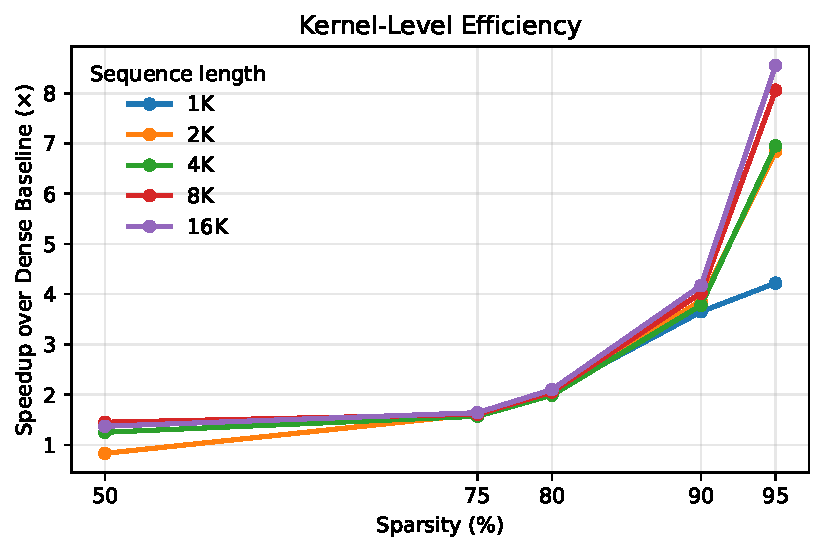
\includegraphics[width=1\linewidth]{figures/kernel_speedup.pdf}
    \caption{Kernel-level wall-clock speedup of the fused block-sparse attention kernel over the dense Flash Attention baseline. Speedup increases with both sequence length and sparsity ratio, reaching $8.6\times$ at 16K tokens with 95\% sparsity.}
    \label{fig:kernel}
\end{figure}

\subsection{Ablation Studies}

We next isolate the two design choices that distinguish Step-dLLM from SparseD: periodic mask refreshing and head-adaptive budget allocation. Unless otherwise specified, all ablations are conducted on LLaDA-1.5 with block size 16.

\paragraph{Refresh frequency.}
Table~\ref{tab:ablation-freq} shows that refresh frequency is a first-order factor. As the refresh interval becomes shorter, both SparseD and Step-dLLM improve, but the gain is consistently larger for Step-dLLM. On GSM8K at 90\% sparsity, SparseD improves from 29.64\% to 43.90\% when moving from one-shot masking ($f{=}1.0$) to frequent refresh ($f{=}0.2$), whereas Step-dLLM improves from 35.18\% to 61.79\%. This confirms that cross-step mask reuse should be local rather than global.

\paragraph{Head-adaptive budget.}
The head-adaptive allocation also contributes independently of refresh. Even under the same one-shot setting ($f{=}1.0$), Step-dLLM still outperforms SparseD, indicating that a better allocation of sparse budget across heads leads to a better mask even before refresh is introduced. For example, Step-dLLM improves GSM8K from 29.64\% to 35.18\% at 90\% sparsity and improves RULER-VT from 86.16\% to 92.32\% at 95\% sparsity. This supports the intuition that different heads exhibit different concentration patterns and should not be forced to share a uniform sparsity rule.

\paragraph{Block size.}
Finally, Table~\ref{tab:ablation-blocksize} shows that Step-dLLM remains stronger than SparseD at both block sizes 16 and 32, and its advantage becomes larger with coarser blocks. At 90\% sparsity on GSM8K, the margin grows from 5.6 points at block size 16 to 22.0 points at block size 32. This trend is expected: when each masking decision removes a larger block, stale masks become more costly, so step-aware refresh and adaptive budget allocation matter even more.

\begin{table}[t]
\centering
\caption{Ablation on mask refresh frequency (LLaDA-1.5, block size 16). Frequency $f$ means the mask is refreshed every $f \times N_{\text{steps}}$ steps; lower $f$ corresponds to more frequent updates. All values are accuracy (\%). \textbf{Bold} marks the best per sparsity level.}
\label{tab:ablation-freq}
\setlength{\tabcolsep}{5pt}
\renewcommand{\arraystretch}{1.15}

\resizebox{\textwidth}{!}{%
\begin{tabular}{@{}ll cccc cccc@{}}
\toprule
\multirow{2.5}{*}{\textbf{Sparsity}} & \multirow{2.5}{*}{\textbf{Metric}}
  & \multicolumn{4}{c}{\textbf{SparseD}}
  & \multicolumn{4}{c}{\textbf{Step-dLLM}} \\
\cmidrule(lr){3-6} \cmidrule(l){7-10}
& & $f{=}1.0$ & $f{=}0.5$ & $f{=}0.3$ & $f{=}0.2$
  & $f{=}1.0$ & $f{=}0.5$ & $f{=}0.3$ & $f{=}0.2$ \\
\midrule

\multirow{3}{*}{95\%}
  & GSM8K    &  9.48 &  6.29 &  5.53 &  6.29 & 16.83 & 16.98 & 17.43 & \textbf{18.80} \\
  & MATH     & 12.00 & 13.80 & 14.20 & 13.60 & 15.40 & 16.00 & 15.40 & \textbf{16.60} \\
  & RULER-VT & 86.16 & 95.40 & 97.04 & 96.64 & 92.32 & 95.36 & 96.36 & \textbf{97.20} \\

\midrule
\multirow{3}{*}{90\%}
  & GSM8K    & 29.64 & 29.72 & 34.19 & 43.90 & 35.18 & 40.64 & 52.24 & \textbf{61.79} \\
  & MATH     & 23.00 & 22.20 & 23.20 & 24.80 & 21.20 & 22.60 & 23.60 & \textbf{26.20} \\
  & RULER-VT & 93.64 & 97.04 & 97.96 & 97.96 & 94.00 & 96.56 & 97.04 & \textbf{97.50} \\

\midrule
\multirow{3}{*}{80\%}
  & GSM8K    & 53.68 & 64.37 & 73.09 & 76.80 & 57.77 & 68.23 & 75.01 & \textbf{77.56} \\
  & MATH     & 29.20 & 31.20 & 32.40 & 34.00 & 31.00 & 32.00 & 33.60 & \textbf{36.40} \\
  & RULER-VT & 94.32 &    -- &    -- &    -- & 98.52 & 96.64 & 97.28 & \textbf{99.88} \\

\bottomrule
\end{tabular}%
}
\end{table}

\begin{table}[t]
\centering
\caption{Ablation on block size (LLaDA-1.5). Accuracy (\%) on short-form benchmarks under block sizes 16 and 32. Step-dLLM consistently outperforms SparseD at both granularities. \textbf{Bold} marks the best per row.}
\label{tab:ablation-blocksize}
\small
\setlength{\tabcolsep}{5pt}
\renewcommand{\arraystretch}{1.12}

\begin{tabular}{llcccc}
\toprule
\multirow{2}{*}{Sparsity} & \multirow{2}{*}{Benchmark}
& \multicolumn{2}{c}{Block size = 16} & \multicolumn{2}{c}{Block size = 32} \\
\cmidrule(lr){3-4} \cmidrule(lr){5-6}
& & SparseD & Step-dLLM & SparseD & Step-dLLM \\
\midrule

\multirow{3}{*}{95\%}
& GSM8K     &  9.86 & \textbf{17.13} &  8.64 & \textbf{19.18} \\
& MATH      &  9.40 & \textbf{13.80} & 10.60 & \textbf{16.20} \\
& HumanEval & 20.12 & \textbf{21.34} & 12.80 & \textbf{23.78} \\
\midrule

\multirow{3}{*}{90\%}
& GSM8K     & 29.64 & \textbf{35.25} & 17.51 & \textbf{39.50} \\
& MATH      & \textbf{20.00} & \textbf{21.60} & 21.60 & \textbf{26.00} \\
& HumanEval & 30.49 & \textbf{32.93} & 28.66 & \textbf{34.15} \\
\midrule

\multirow{3}{*}{80\%}
& GSM8K     & 53.68 & \textbf{58.38} & 50.87 & \textbf{63.23} \\
& MATH      & \textbf{28.20} & 27.60 & 31.60 & 31.20 \\
& HumanEval & 36.59 & \textbf{37.20} & 37.80 & \textbf{39.12} \\

\bottomrule
\end{tabular}
\end{table}



% \subsection{Main Results}
% %We present the inference accuracy of Step-dLLM and all baselines on Llada-1.5 and Dream-7B across all benchmarks, as shown in Table 1.
% We evaluate Step-dLLM on two representative diffusion LLMs, LlaDA-1.5 and Dream-7B-Instruct (Table~\ref{tab:main-bs16-llada} and Table~\ref{tab:main-bs16-dream}), covering short-form reasoning/code benchmarks (GSM8K, MATH, HumanEval) and long-context benchmarks (NIAH, RULER). All methods are compared under the same sparsity budgets (50\% 80\% 90\% 95\%) against Dense, StreamingLLM, and SparseD. Overall, StreamingLLM exhibits a severe quality collapse on diffusion LLMs, while Step-dLLM is consistently more robust—especially at high sparsity (90\%–95\%)—and preserves strong long-context performance, validating the benefit of step-aware sparse updates and global budget allocation under denoising-step dynamics.

% Table~\ref{tab:main-bs16-llada} and Table~\ref{tab:main-bs16-dream} show that Step-dLLM is consistently more robust than SparseD at high sparsity(90\%–95\%) on both LlaDA-1.5 and Dream-7B-Instruct, because it aligns the sparsity pattern with DLLMs step dynamics: unlike SparseD’s largely step-agnostic masking, Step-dLLM leverages the fact that attention-score structure is correlated across denoising steps but shifts across stages, so it reuses masks when cross-step similarity is high and refreshes them when the step/stage distribution changes. This step-aware, stage-aware mask updating prevents the “stale mask” failure mode under aggressive sparsity, thereby preserving reasoning/code accuracy while maintaining long-context quality on NIAH/RULER.

% Also, the tables demonstrate that Step-dLLM delivers a better accuracy–efficiency tradeoff than SparseD at high sparsity (90\%–95\%) and avoids the quality collapse of traditional AR mathod, like StreamingLLM, on DLLMs.


% Model: LLaDA-1.5, Dream-7B-Instruct

% Bench: MATH500, Human-eval, RULER, NIAH, GSM8K

% Baseline: StreamingLLM, SparseD, FastDLLM

% \begin{itemize}
% \item Dense
% \item + StreamingLLM
% \item + SparseD
% % \item + OPT1
% \item + Ours
% \item (optional) fastdllm
% \end{itemize}

% Setting:
% Sparsity: 95\%, 90\%, 80\%, 50\%

% Step updating: 1/2, 1/3, 1/5, 1/10, 0

% Block Size: 16, 32

% \begin{table}[t]
\centering
\caption{Main results on LLaDA-1.5 with block size 16. All values are accuracy (\%). \textbf{Bold} marks the best result per sparsity level (excluding Dense).}
\label{tab:main-bs16-llada}
\setlength{\tabcolsep}{3.5pt}
\renewcommand{\arraystretch}{1.15}

\resizebox{\textwidth}{!}{%
\begin{tabular}{@{}ll ccc ccccccccc ccccc@{}}
\toprule
\multirow{2.5}{*}{\textbf{Method}} & \multirow{2.5}{*}{\textbf{Sparsity}}
  & \multicolumn{3}{c}{\textbf{Short-form}}
  & \multicolumn{8}{c}{\textbf{NIAH}}
  & \multicolumn{5}{c}{\textbf{RULER}} \\
\cmidrule(lr){3-5} \cmidrule(lr){6-13} \cmidrule(l){14-18}
& & GSM8K & Math & HumanE
  & $\text{S}_1$ & $\text{S}_2$ & $\text{S}_3$
  & $\text{MK}_1$ & $\text{MK}_2$ & $\text{MK}_3$
  & MQ & MV
  & VT & CWE & FWE & QS & QH \\
\midrule

Dense & --
  & \textbf{81.04} & \textbf{37.20} & \textbf{40.24}
  & \textbf{100.0} & \textbf{100.0} & \textbf{100.0} & \textbf{100.0}
  & \textbf{100.0} & \textbf{100.0} & \textbf{100.0} & \textbf{100.0}
  & \textbf{100.0} & \textbf{52.40} & \textbf{64.20} & \textbf{91.30} & \textbf{76.00} \\

\midrule
\multirow{3}{*}{StreamingLLM}
  & 50\% & 74.07 & \textbf{38.20} & 39.02
    & 20.80 & 20.20 & 18.40 & 21.20 & 20.40 & 15.40 & 19.20 & 14.40
    & 30.60 & 13.40 & 73.80 & 81.65 & 44.40 \\
  & 80\% & 19.11 & 13.60 & 19.51
    & 5.00 & 2.40 & 1.40 & 3.40 & 3.60 & 0.00 & 2.10 & 2.10
    & 6.56 & 3.02 & 76.27 & 20.48 & 22.40 \\
  & 90\% & 0.08 & 0.00 & 2.43
    & 0.00 & 0.00 & 0.00 & 0.00 & 0.00 & 0.00 & 0.00 & 0.00
    & 0.00 & 2.12 & 0.00 & 0.27 & 0.00 \\

\midrule
\multirow{4}{*}{SparseD}
  & 50\% & 80.59 & 37.40 & 42.68
    & \textbf{100.0} & \textbf{100.0} & \textbf{100.0} & \textbf{100.0}
    & \textbf{100.0} & \textbf{100.0} & \textbf{100.0} & \textbf{100.0}
    & \textbf{99.88} & 52.26 & \textbf{61.40} & \textbf{83.17} & 77.60 \\
  & 80\% & 53.68 & \textbf{28.20} & 36.59
    & \textbf{100.0} & \textbf{100.0} & 71.20 & \textbf{100.0}
    & \textbf{100.0} & 74.20 & 85.85 & 79.10
    & 94.28 & \textbf{57.80} & 45.40 & 83.48 & 77.80 \\
  & 90\% & 29.64 & 20.00 & 30.49
    & \textbf{100.0} & \textbf{100.0} & 76.60 & \textbf{100.0}
    & 99.80 & 77.20 & 82.85 & 80.60
    & 93.32 & 34.56 & 42.07 & 83.13 & 76.00 \\
  & 95\% & 9.86 & 9.40 & 20.12
    & \textbf{100.0} & \textbf{100.0} & 79.40 & \textbf{100.0}
    & \textbf{100.0} & 78.20 & 81.80 & 81.10
    & 86.64 & 39.92 & 39.00 & \textbf{81.97} & \textbf{73.60} \\

\midrule
\multirow{4}{*}{\textbf{Step-dLLM}}
  & 50\% & \textbf{82.71} & 36.80 & \textbf{42.68}
    & \textbf{100.0} & \textbf{100.0} & \textbf{100.0} & \textbf{100.0}
    & \textbf{100.0} & \textbf{100.0} & \textbf{100.0} & \textbf{100.0}
    & 99.60 & \textbf{53.16} & 60.87 & 83.03 & \textbf{78.60} \\
  & 80\% & \textbf{58.38} & 27.60 & \textbf{37.20}
    & \textbf{100.0} & \textbf{100.0} & \textbf{100.0} & \textbf{100.0}
    & 99.80 & \textbf{99.60} & \textbf{99.90} & \textbf{98.60}
    & \textbf{98.52} & 56.46 & \textbf{51.73} & \textbf{83.73} & \textbf{78.20} \\
  & 90\% & \textbf{35.25} & \textbf{21.60} & \textbf{32.93}
    & \textbf{100.0} & \textbf{100.0} & \textbf{100.0} & \textbf{100.0}
    & \textbf{100.0} & \textbf{97.60} & \textbf{99.65} & \textbf{95.90}
    & \textbf{94.00} & \textbf{54.16} & \textbf{46.80} & \textbf{83.48} & \textbf{76.40} \\
  & 95\% & \textbf{17.13} & \textbf{13.80} & \textbf{21.34}
    & \textbf{100.0} & \textbf{100.0} & \textbf{98.80} & \textbf{100.0}
    & \textbf{100.0} & \textbf{88.40} & \textbf{95.25} & \textbf{92.30}
    & \textbf{92.32} & \textbf{44.76} & \textbf{44.07} & 81.37 & 71.40 \\
\bottomrule
\end{tabular}%
}
\end{table}

% \begin{table}[t]
\centering
\caption{Main results on Dream-7B-Instruct with block size 16. All values are accuracy (\%). \textbf{Bold} marks the best result per sparsity level (excluding Dense).}
\label{tab:main-bs16-dream}
\setlength{\tabcolsep}{3.5pt}
\renewcommand{\arraystretch}{1.15}

\resizebox{\textwidth}{!}{%
\begin{tabular}{@{}ll ccc ccccccccc ccccc@{}}
\toprule
\multirow{2.5}{*}{\textbf{Method}} & \multirow{2.5}{*}{\textbf{Sparsity}}
  & \multicolumn{3}{c}{\textbf{Short-form}}
  & \multicolumn{8}{c}{\textbf{NIAH}}
  & \multicolumn{5}{c}{\textbf{RULER}} \\
\cmidrule(lr){3-5} \cmidrule(lr){6-13} \cmidrule(l){14-18}
& & GSM8K & Math & HumanE
  & $\text{S}_1$ & $\text{S}_2$ & $\text{S}_3$
  & $\text{MK}_1$ & $\text{MK}_2$ & $\text{MK}_3$
  & MQ & MV
  & VT & CWE & FWE & QS & QH \\
\midrule

Dense & --
  & \textbf{77.41} & \textbf{45.60} & --
  & \textbf{100.0} & \textbf{100.0} & \textbf{91.00} & \textbf{98.00}
  & \textbf{99.80} & \textbf{77.60} & \textbf{97.70} & \textbf{96.40}
  & \textbf{96.32} & \textbf{87.28} & \textbf{79.47} & \textbf{79.57} & \textbf{64.00} \\

\midrule
\multirow{3}{*}{StreamingLLM}
  & 50\% & 38.13 & 8.80 & 42.70
    & 10.00 & 11.00 & 9.00 & 11.00 & 8.80 & 12.40 & 8.75 & 10.30
    & 13.40 & 43.34 & 37.73 & \textbf{81.40} & 33.00 \\
  & 80\% & 19.56 & 10.40 & 25.00
    & 1.80 & 2.80 & 1.40 & 3.20 & 1.20 & 0.00 & 1.95 & 2.40
    & 0.36 & 4.54 & 4.33 & 19.18 & 19.60 \\
  & 90\% & 0.00 & 0.00 & 2.44
    & 0.00 & 0.00 & 0.00 & 0.00 & 0.00 & 0.00 & 0.00 & 0.00
    & 0.00 & 0.00 & 0.00 & 0.00 & 0.00 \\

\midrule
\multirow{4}{*}{SparseD}
  & 50\% & 70.50 & 43.60 & 56.10
    & \textbf{100.0} & \textbf{100.0} & 90.20 & \textbf{98.00} & 99.40 & \textbf{75.80}
    & \textbf{97.45} & 97.40
    & 96.28 & \textbf{85.16} & \textbf{75.80} & 80.37 & \textbf{64.60} \\
  & 80\% & 49.81 & 37.80 & 53.66
    & \textbf{100.0} & \textbf{99.80} & 47.20 & \textbf{98.80} & \textbf{99.80} & 46.80
    & 60.05 & 69.30
    & 95.44 & 71.76 & \textbf{71.77} & \textbf{79.50} & 61.00 \\
  & 90\% & 22.21 & 28.80 & 43.90
    & \textbf{100.0} & \textbf{100.0} & 44.60 & \textbf{98.80} & \textbf{99.80} & \textbf{44.80}
    & \textbf{59.45} & \textbf{69.00}
    & 92.20 & 54.72 & 67.53 & 78.45 & \textbf{61.60} \\
  & 95\% & 4.40 & 14.80 & 31.10
    & \textbf{100.0} & \textbf{100.0} & \textbf{40.80} & \textbf{98.40} & 99.40 & \textbf{37.40}
    & \textbf{53.95} & \textbf{66.85}
    & 78.64 & 43.84 & 62.26 & 77.60 & 60.00 \\

\midrule
\multirow{4}{*}{\textbf{Step-dLLM}}
  & 50\% & \textbf{71.80} & \textbf{44.00} & \textbf{58.54}
    & \textbf{100.0} & \textbf{100.0} & \textbf{90.50} & 97.80 & \textbf{99.80} & 75.60
    & 97.25 & \textbf{97.50}
    & \textbf{96.40} & 83.24 & 75.53 & 79.80 & 63.80 \\
  & 80\% & \textbf{52.39} & \textbf{38.60} & \textbf{54.27}
    & \textbf{100.0} & \textbf{99.80} & \textbf{69.00} & 98.20 & \textbf{99.80} & \textbf{65.40}
    & \textbf{74.10} & \textbf{78.40}
    & \textbf{96.04} & \textbf{73.24} & 71.13 & 78.53 & \textbf{61.80} \\
  & 90\% & \textbf{32.68} & \textbf{32.00} & \textbf{50.00}
    & \textbf{100.0} & 99.80 & \textbf{47.00} & 97.20 & \textbf{99.80} & 39.80
    & 57.30 & 68.05
    & \textbf{94.68} & \textbf{59.58} & \textbf{68.26} & \textbf{79.03} & 60.20 \\
  & 95\% & \textbf{15.31} & \textbf{19.20} & \textbf{35.98}
    & \textbf{100.0} & 99.60 & 37.20 & 95.60 & \textbf{99.60} & 33.60
    & 52.30 & 60.95
    & \textbf{82.08} & \textbf{46.90} & \textbf{62.87} & \textbf{77.83} & \textbf{61.40} \\
\bottomrule
\end{tabular}%
}
\end{table}

% %\begin{table}[t]
\centering
\caption{Long-context results on LLaDA-1.5 with block size 16 (NIAH and RULER benchmarks). All values are accuracy (\%). \textbf{Bold} marks the best result per sparsity level (excluding Dense).}
\label{tab:main-bs16-llada-long}
\setlength{\tabcolsep}{3.5pt}
\renewcommand{\arraystretch}{1.15}

\resizebox{\textwidth}{!}{%
\begin{tabular}{@{}ll cccccccc ccccc@{}}
\toprule
\multirow{2.5}{*}{\textbf{Method}} & \multirow{2.5}{*}{\textbf{Sparsity}}
  & \multicolumn{8}{c}{\textbf{NIAH}}
  & \multicolumn{5}{c}{\textbf{RULER}} \\
\cmidrule(lr){3-10} \cmidrule(l){11-15}
& & $\text{S}_1$ & $\text{S}_2$ & $\text{S}_3$
  & $\text{MK}_1$ & $\text{MK}_2$ & $\text{MK}_3$
  & MQ & MV
  & VT & CWE & FWE & QS & QH \\
\midrule

Dense & --
  & \textbf{100.0} & \textbf{100.0} & \textbf{100.0} & \textbf{100.0}
  & \textbf{100.0} & \textbf{100.0} & \textbf{100.0} & \textbf{100.0}
  & \textbf{100.0} & \textbf{52.40} & \textbf{64.20} & \textbf{91.30} & \textbf{76.00} \\

\midrule
\multirow{3}{*}{StreamingLLM}
  & 50\% & 20.80 & 20.20 & 18.40 & 21.20 & 20.40 & 15.40 & 19.20 & 14.40
    & 30.60 & 13.40 & 73.80 & 81.65 & 44.40 \\
  & 80\% & 5.00 & 2.40 & 1.40 & 3.40 & 3.60 & 0.00 & 2.10 & 2.10
    & 6.56 & 3.02 & 76.27 & 20.48 & 22.40 \\
  & 90\% & 0.00 & 0.00 & 0.00 & 0.00 & 0.00 & 0.00 & 0.00 & 0.00
    & 0.00 & 2.12 & 0.00 & 0.27 & 0.00 \\

\midrule
\multirow{4}{*}{SparseD}
  & 50\% & \textbf{100.0} & \textbf{100.0} & \textbf{100.0} & \textbf{100.0}
    & \textbf{100.0} & \textbf{100.0} & \textbf{100.0} & \textbf{100.0}
    & \textbf{99.88} & 52.26 & \textbf{61.40} & \textbf{83.17} & 77.60 \\
  & 80\% & \textbf{100.0} & \textbf{100.0} & 71.20 & \textbf{100.0}
    & \textbf{100.0} & 74.20 & 85.85 & 79.10
    & 94.28 & \textbf{57.80} & 45.40 & 83.48 & 77.80 \\
  & 90\% & \textbf{100.0} & \textbf{100.0} & 76.60 & \textbf{100.0}
    & 99.80 & 77.20 & 82.85 & 80.60
    & 93.32 & 34.56 & 42.07 & 83.13 & 76.00 \\
  & 95\% & \textbf{100.0} & \textbf{100.0} & 79.40 & \textbf{100.0}
    & \textbf{100.0} & 78.20 & 81.80 & 81.10
    & 86.64 & 39.92 & 39.00 & \textbf{81.97} & \textbf{73.60} \\

\midrule
\multirow{4}{*}{\textbf{Step-dLLM}}
  & 50\% & \textbf{100.0} & \textbf{100.0} & \textbf{100.0} & \textbf{100.0}
    & \textbf{100.0} & \textbf{100.0} & \textbf{100.0} & \textbf{100.0}
    & 99.60 & \textbf{53.16} & 60.87 & 83.03 & \textbf{78.60} \\
  & 80\% & \textbf{100.0} & \textbf{100.0} & \textbf{100.0} & \textbf{100.0}
    & 99.80 & \textbf{99.60} & \textbf{99.90} & \textbf{98.60}
    & \textbf{98.52} & 56.46 & \textbf{51.73} & \textbf{83.73} & \textbf{78.20} \\
  & 90\% & \textbf{100.0} & \textbf{100.0} & \textbf{100.0} & \textbf{100.0}
    & \textbf{100.0} & \textbf{97.60} & \textbf{99.65} & \textbf{95.90}
    & \textbf{94.00} & \textbf{54.16} & \textbf{46.80} & \textbf{83.48} & \textbf{76.40} \\
  & 95\% & \textbf{100.0} & \textbf{100.0} & \textbf{98.80} & \textbf{100.0}
    & \textbf{100.0} & \textbf{88.40} & \textbf{95.25} & \textbf{92.30}
    & \textbf{92.32} & \textbf{44.76} & \textbf{44.07} & 81.37 & 71.40 \\
\bottomrule
\end{tabular}%
}
\end{table}





% % \subsection{Efficiency}
% Sequence length (total): 1K, 2K, 4K (@JUNPAN)

% Kernel-level: all heads block-wise sparse attention

% e2e: + step-update + sparse attn

% Figure~\ref{fig:kernel}
% \begin{figure}[t]
%     \centering
%     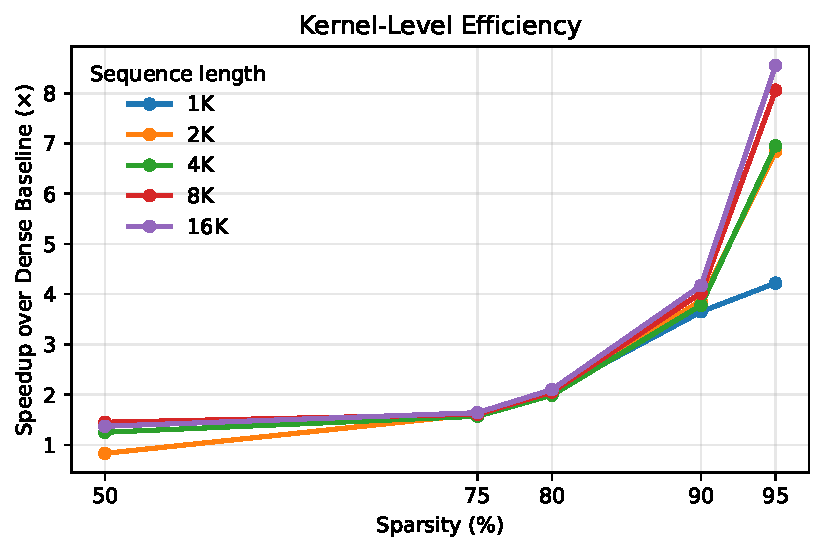
\includegraphics[width=1\linewidth]{figures/kernel_speedup.pdf}
%     \caption{Kernel-level speedup over the dense baseline under different sparsity levels and sequence lengths. Larger gains are achieved in longer-context and higher-sparsity regimes.}
%     \label{fig:kernel}
% \end{figure}
% summarizes the kernel-level efficiency of our Step-dLLM implementation. Specifically, we develop a customized CUDA kernel that fuses step-aware mask updating with block-wise sparse attention, and benchmark its end-to-end runtime under different sequence lengths (from 1K to 16K) and sparsity budgets. Across all settings, the proposed kernel achieves substantial speedups over the dense baseline, with gains increasing as either the sequence length grows or the sparsity becomes more aggressive, reaching up to ~8× speedup at long-context and high-sparsity regimes. This shows that Step-dLLM’s step-aware sparse attention is not only algorithmically effective but also practically efficient at the kernel level.

% %\begin{table}[H]
  \centering
  \caption{Add caption}
  \label{tab:main-kernel-level}

  \small
  \setlength{\tabcolsep}{4pt}
  \renewcommand{\arraystretch}{1.08}

  \resizebox{\columnwidth}{!}{%
    \begin{tabular}{ccccc}
    \toprule
    Kernel Size & Sparsity & Baseline (dense) & Ours & Speedup \\
    \midrule

    \multirow{5}{*}{1K}
      & 95\% & 0.053041 & 0.01257000 & 4.22 \\
      & 90\% & 0.053041 & 0.01452900 & 3.65 \\
      & 80\% & 0.053041 & 0.02579500 & 2.06 \\
      & 75\% & 0.053041 & 0.03299900 & 1.61 \\
      & 50\% & 0.053041 & 0.06417000 & 0.83 \\
    \midrule

    \multirow{5}{*}{2K}
      & 95\% & 0.193364 & 0.02827213 & 6.84 \\
      & 90\% & 0.193364 & 0.04997750 & 3.87 \\
      & 80\% & 0.193364 & 0.09559138 & 2.02 \\
      & 75\% & 0.193364 & 0.12004263 & 1.61 \\
      & 50\% & 0.193364 & 0.23373875 & 0.83 \\
    \midrule

    \multirow{5}{*}{4K}
      & 95\% & 0.763358 & 0.10975700 & 6.95 \\
      & 90\% & 0.763358 & 0.20190700 & 3.78 \\
      & 80\% & 0.763358 & 0.38442200 & 1.99 \\
      & 75\% & 0.763358 & 0.48581000 & 1.57 \\
      & 50\% & 0.763358 & 0.61274000 & 1.25 \\
    \midrule

    \multirow{5}{*}{8K}
      & 95\% & 2.952540 & 0.36623300 & 8.06 \\
      & 90\% & 2.952540 & 0.73515000 & 4.02 \\
      & 80\% & 2.952540 & 1.43898800 & 2.05 \\
      & 75\% & 2.952540 & 1.83316500 & 1.61 \\
      & 50\% & 2.952540 & 2.03316500 & 1.45 \\
    \midrule

    \multirow{5}{*}{16K}
      & 95\% & 11.837924 & 1.38469300 & 8.55 \\
      & 90\% & 11.837924 & 2.84201000 & 4.17 \\
      & 80\% & 11.837924 & 5.63847300 & 2.10 \\
      & 75\% & 11.837924 & 7.21230000 & 1.64 \\
      & 50\% & 11.837924 & 8.61280000 & 1.37 \\
    \bottomrule
    \end{tabular}%
  }
\end{table}

% \subsection{Ablation Study}

% 1. Block size: 8, 16, 32

% We also did further ablation study for block size 32, since the StreamingLLM doesn't have block size, we only compare the results of SparseD and Ours. The results of experimention are shown in table 4 & table 5:

% %\begin{table}[t]
\centering
\caption{Main results on LLaDA-1.5 with block size 32. All values are accuracy (\%). \textbf{Bold} marks the best result per sparsity level (excluding Dense).}
\label{tab:main-bs32-llada}
\setlength{\tabcolsep}{3.5pt}
\renewcommand{\arraystretch}{1.15}

\resizebox{\textwidth}{!}{%
\begin{tabular}{@{}ll ccc ccccccccc ccccc@{}}
\toprule
\multirow{2.5}{*}{\textbf{Method}} & \multirow{2.5}{*}{\textbf{Sparsity}}
  & \multicolumn{3}{c}{\textbf{Short-form}}
  & \multicolumn{8}{c}{\textbf{NIAH}}
  & \multicolumn{5}{c}{\textbf{RULER}} \\
\cmidrule(lr){3-5} \cmidrule(lr){6-13} \cmidrule(l){14-18}
& & GSM8K & Math & HumanE
  & $\text{S}_1$ & $\text{S}_2$ & $\text{S}_3$
  & $\text{MK}_1$ & $\text{MK}_2$ & $\text{MK}_3$
  & MQ & MV
  & VT & CWE & FWE & QS & QH \\
\midrule

Dense & --
  & \textbf{81.04} & \textbf{37.20} & \textbf{40.24}
  & \textbf{100.0} & \textbf{100.0} & \textbf{100.0} & \textbf{100.0}
  & \textbf{100.0} & \textbf{100.0} & \textbf{100.0} & \textbf{100.0}
  & \textbf{100.0} & \textbf{52.40} & \textbf{64.20} & \textbf{91.30} & \textbf{76.00} \\

\midrule
\multirow{4}{*}{SparseD}
  & 50\% & \textbf{73.09} & \textbf{40.60} & 40.85
    & \textbf{100.0} & \textbf{100.0} & \textbf{100.0} & \textbf{100.0}
    & \textbf{100.0} & \textbf{100.0} & -- & --
    & \textbf{100.0} & 49.00 & \textbf{66.93} & \textbf{83.43} & 77.40 \\
  & 80\% & 46.17 & \textbf{31.60} & 37.80
    & \textbf{100.0} & \textbf{100.0} & 87.60 & \textbf{100.0}
    & \textbf{100.0} & 93.60 & -- & --
    & 99.56 & 48.26 & 52.73 & \textbf{83.77} & 77.00 \\
  & 90\% & 17.29 & 21.60 & 28.66
    & \textbf{100.0} & \textbf{100.0} & 88.00 & \textbf{100.0}
    & \textbf{100.0} & 94.00 & 98.00 & 90.80
    & 93.32 & 46.64 & 49.93 & \textbf{84.23} & 75.40 \\
  & 95\% & 12.66 & 10.60 & 12.80
    & \textbf{100.0} & \textbf{100.0} & \textbf{88.20} & \textbf{100.0}
    & \textbf{100.0} & 92.80 & \textbf{98.55} & 88.80
    & 63.00 & 43.44 & 30.80 & 83.45 & 73.60 \\

\midrule
\multirow{4}{*}{\textbf{Step-dLLM}}
  & 50\% & \textbf{73.09} & 40.40 & \textbf{42.07}
    & \textbf{100.0} & \textbf{100.0} & \textbf{100.0} & \textbf{100.0}
    & \textbf{100.0} & \textbf{100.0} & -- & --
    & 99.92 & \textbf{49.14} & 63.07 & 82.50 & \textbf{77.60} \\
  & 80\% & \textbf{57.39} & 31.20 & \textbf{39.12}
    & \textbf{100.0} & \textbf{100.0} & \textbf{94.80} & \textbf{100.0}
    & \textbf{100.0} & \textbf{96.80} & -- & --
    & \textbf{99.80} & \textbf{51.28} & \textbf{57.00} & 83.23 & \textbf{77.20} \\
  & 90\% & \textbf{40.86} & \textbf{26.00} & \textbf{34.15}
    & \textbf{100.0} & \textbf{100.0} & \textbf{88.20} & \textbf{100.0}
    & \textbf{100.0} & \textbf{95.40} & \textbf{98.60} & \textbf{93.65}
    & \textbf{98.48} & \textbf{50.02} & \textbf{50.13} & 82.37 & \textbf{76.40} \\
  & 95\% & \textbf{21.60} & \textbf{16.20} & \textbf{23.78}
    & \textbf{100.0} & \textbf{100.0} & 87.80 & \textbf{100.0}
    & \textbf{100.0} & \textbf{94.00} & 98.50 & \textbf{91.00}
    & \textbf{89.28} & \textbf{47.24} & \textbf{44.67} & \textbf{83.53} & \textbf{74.80} \\
\bottomrule
\end{tabular}%
}
\end{table}

% %\begin{table}[t]
\centering
\caption{Main results on Dream-7B-Instruct with block size 32. All values are accuracy (\%). \textbf{Bold} marks the best result per sparsity level (excluding Dense).}
\label{tab:main-bs32-dream}
\setlength{\tabcolsep}{3.5pt}
\renewcommand{\arraystretch}{1.15}

\resizebox{\textwidth}{!}{%
\begin{tabular}{@{}ll ccc ccccccccc ccccc@{}}
\toprule
\multirow{2.5}{*}{\textbf{Method}} & \multirow{2.5}{*}{\textbf{Sparsity}}
  & \multicolumn{3}{c}{\textbf{Short-form}}
  & \multicolumn{8}{c}{\textbf{NIAH}}
  & \multicolumn{5}{c}{\textbf{RULER}} \\
\cmidrule(lr){3-5} \cmidrule(lr){6-13} \cmidrule(l){14-18}
& & GSM8K & Math & HumanE
  & $\text{S}_1$ & $\text{S}_2$ & $\text{S}_3$
  & $\text{MK}_1$ & $\text{MK}_2$ & $\text{MK}_3$
  & MQ & MV
  & VT & CWE & FWE & QS & QH \\
\midrule

Dense & --
  & \textbf{77.41} & \textbf{45.60} & --$^\dagger$
  & \textbf{100.0} & \textbf{100.0} & \textbf{91.00} & \textbf{98.00}
  & \textbf{99.80} & \textbf{77.60} & \textbf{97.70} & \textbf{96.40}
  & \textbf{96.32} & \textbf{87.28} & \textbf{79.47} & \textbf{79.57} & \textbf{64.00} \\

\midrule
\multirow{4}{*}{SparseD}
  & 50\% & \textbf{73.09} & 42.00 & 56.10
    & \textbf{100.0} & 99.80 & 92.40 & \textbf{98.40} & \textbf{99.80} & 76.00
    & \textbf{97.55} & \textbf{98.05}
    & 96.20 & \textbf{84.48} & \textbf{76.40} & 79.73 & \textbf{64.00} \\
  & 80\% & 46.17 & 39.20 & 53.05
    & \textbf{100.0} & \textbf{99.80} & 75.00 & \textbf{98.60} & \textbf{99.80} & 70.60
    & 90.70 & 97.75
    & 94.12 & 68.64 & 72.07 & \textbf{80.57} & \textbf{64.60} \\
  & 90\% & 17.29 & 29.20 & \textbf{49.39}
    & \textbf{100.0} & \textbf{99.80} & \textbf{72.60} & \textbf{98.00} & \textbf{99.80} & 68.80
    & \textbf{89.80} & \textbf{96.95}
    & 80.60 & 53.80 & 67.87 & \textbf{79.40} & \textbf{64.40} \\
  & 95\% & 12.66 & 11.60 & 21.34
    & \textbf{100.0} & \textbf{97.80} & \textbf{70.20} & \textbf{90.20} & 99.40 & 64.20
    & \textbf{78.95} & \textbf{81.85}
    & \textbf{24.52} & 44.38 & \textbf{62.60} & 77.87 & \textbf{60.60} \\

\midrule
\multirow{4}{*}{\textbf{Step-dLLM}}
  & 50\% & \textbf{73.09} & \textbf{44.60} & \textbf{58.54}
    & \textbf{100.0} & \textbf{100.0} & \textbf{93.20} & \textbf{98.40} & \textbf{99.80} & \textbf{77.20}
    & 96.00 & 97.95
    & \textbf{96.52} & 83.28 & 76.13 & \textbf{80.18} & 63.80 \\
  & 80\% & \textbf{57.39} & \textbf{39.80} & \textbf{53.66}
    & \textbf{100.0} & \textbf{99.80} & \textbf{75.60} & 98.20 & \textbf{99.80} & \textbf{71.20}
    & \textbf{90.85} & \textbf{98.25}
    & \textbf{95.76} & \textbf{72.10} & \textbf{72.20} & 79.17 & 63.20 \\
  & 90\% & \textbf{40.86} & \textbf{30.60} & 47.56
    & \textbf{100.0} & \textbf{99.80} & 72.20 & 94.60 & \textbf{99.80} & \textbf{70.00}
    & 88.15 & 96.25
    & \textbf{91.56} & \textbf{59.36} & \textbf{69.60} & 78.67 & 63.00 \\
  & 95\% & \textbf{21.60} & \textbf{20.40} & \textbf{33.54}
    & \textbf{100.0} & 86.80 & 67.40 & 83.60 & \textbf{99.60} & \textbf{67.60}
    & 74.10 & 74.40
    & 20.40 & \textbf{47.07} & 59.93 & 75.77 & \textbf{60.60} \\
\bottomrule
\multicolumn{18}{@{}l}{\footnotesize $^\dagger$\,HumanEval not evaluated for Dream-7B-Instruct under dense inference.}
\end{tabular}%
}
\end{table}


% 2. Step update frequency: 

% 3. OPT1, OPT2

% 4. Accuracy \& efficiency tradeoff


\section{Conclusion}

We presented \textbf{Step-dLLM}, a sparse attention framework designed for the unique dynamics of diffusion language models. Our analysis reveals two properties that prior methods overlook: attention patterns in DLMs are locally consistent but not globally stationary across denoising steps, and different attention heads exhibit markedly different concentration behaviors. Step-dLLM exploits both observations through three integrated components: cross-step mask reuse with periodic refresh at anchor steps, a head-adaptive budget that allocates sparse computation according to each head's cumulative saliency, and fused Triton kernels that translate algorithmic savings into wall-clock speedups. Extensive experiments on LLaDA-1.5 and Dream-7B-Instruct across mathematical reasoning, code generation, and long-context retrieval benchmarks show that Step-dLLM consistently achieves the best accuracy--sparsity trade-off among sparse baselines, with advantages that grow under high sparsity---where stale masks are most harmful---and on long-context tasks, where the set of salient positions shifts substantially during denoising. At the kernel level, the fused block-sparse attention kernel delivers up to $8.6\times$ speedup over dense Flash Attention at 95\% sparsity.

Several directions remain open. The current anchor schedule uses a fixed refresh interval~$\Delta$; an adaptive strategy that triggers re-anchoring when the KL divergence between consecutive steps exceeds a threshold could better track abrupt attention transitions while further reducing the number of full-attention computations. Additionally, exploring whether the head-adaptive budget can be extended to full head pruning---entirely skipping heads whose saliency falls below a threshold at certain denoising stages---may yield further efficiency gains. Finally, integrating Step-dLLM with complementary acceleration techniques such as semi-autoregressive block decoding and step-reduction schedules is a promising avenue for compounding speedups in diffusion language model inference. More broadly, the anchor-refresh paradigm---periodically refreshing a sparse mask at selected steps to track shifting attention structure---is not specific to masked discrete diffusion: it may generalize to continuous diffusion transformers, multi-round editing, or any iterative generation process where attention patterns evolve across steps.


\bibliography{example_paper}
\bibliographystyle{plainnat}

%%%%%%%%%%%%%%%%%%%%%%%%%%%%%%%%%%%%%%%%%%%%%%%%%%%%%%%%%%%%%%%%%%%%%%%%%%%%%%%
% APPENDIX
%%%%%%%%%%%%%%%%%%%%%%%%%%%%%%%%%%%%%%%%%%%%%%%%%%%%%%%%%%%%%%%%%%%%%%%%%%%%%%%
\appendix
\section{Appendix}

% You can have as much text here as you want. There is no page limit for the
% technical appendices.

%%%%%%%%%%%%%%%%%%%%%%%%%%%%%%%%%%%%%%%%%%%%%%%%%%%%%%%%%%%%%%%%%%%%%%%%%%%%%%%

% \newpage
% \input{checklist.tex}

\end{document}
